\documentclass[
    DIV12,
    cleardouble=plain,
    headings=normal,
    pdftex,
    headexclude,footexclude,
    final
]{scrreprt}

\usepackage{spreadtab}
\usepackage{xspace}
\usepackage{ngerman}
\usepackage[utf8]{inputenc}
%\usepackage[T1]{fontenc}
\usepackage[pdftex]{graphicx}
\usepackage[bookmarks]{hyperref}
\usepackage{scrpage2}
\usepackage{longtable}
\usepackage{caption}
\usepackage{pgfplots}
\usepackage{float}
\usepackage{xcolor}
\usepackage{colortbl}
\usepackage{relsize}
\usepackage{fancyvrb}

\usepackage{geometry}
\usepackage{multicol}
\usepackage{multido}
\usepackage{hyperref}
\usepackage{listings}

\graphicspath{{./}{./Pics/}}

% #################################################################

\hyphenation{Cha-otn-gsch-werl}
\setlength\headheight{1.75cm}

\ihead{\small{Hochschule Hof}}
\chead{}
\ohead{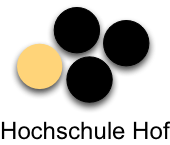
\includegraphics[height=0.05\textheight]{LogoGelb.png}}
\pagestyle{scrheadings}


\setcounter{secnumdepth}{5}
\setcounter{tocdepth}{5}
\renewcommand{\arraystretch}{1}

\parskip0.5\baselineskip plus 0.125\baselineskip minus 0.25\baselineskip
\parindent0em

% #################################################################

\def\SECH{S\kern-.075em \lower.5ex\hbox{E}\kern-0.05em CH\xspace}
\def\SEACH{S\kern-.075em \lower.5ex\hbox{E}\kern-0.05em ACH\xspace}

% #################################################################

%\automark[section]{chapter}

\titlehead{\begin{center}
\includegraphics[width=5cm]{fh_logo}\end{center}}
\title{
  \SECH--Tag--EEXCESS--Browser \\[1em]
  Programming Guide\\
Spezifikation, Konstruktion
}

\author{Prof. Dr. Peter Stöhr \and Gottfried von Recum \and Alexander Pöhlmann \and Tim Pohrer \and Lothar Mödl \and Burak Erol \and Brian Mairhörmann \and Andreas Netsch \and Philipp Winterholler \and Patrick Büttner \and Andreas Ziemer}
\date{Version 0.1.1}

% #################################################################


\begin{document}
\maketitle
\pagenumbering{Roman}
\tableofcontents

\listoftables

\newpage
\pagenumbering{arabic}

\part*{Einleitung}
\chapter*{�ber dieses Dokument}

Dieses Dokument dient als Container f�r die im Lauf der
Arbeiten an dem \SECH--Projekt entstehenden Unterlagen. Die
Quellen f�r dieses Dokument liegen auf GutHub unter der URL
\url{https://github.com/SECH-App}.

Das Dokument muss von den bearbeitenden Gruppen parallel zu den
Entwicklungsarbeiten weiterentwickelt werden. 

Aktuell beschreibt das Dokument den Entwicklungsstand zum
Wintersemester 2015 und besteht aus folgenden Teilen:
\begin{enumerate}
     \item Einf�hrung in die Programmierung eines EEXCESS Clients.
     \item Spezifikation der beiden Teilsysteme.
     \item Konstruktion der beiden Teilsysteme.
\end{enumerate}


\chapter{\SECH--Browser}

\section{Projektziel}
Das Web besteht aus einer Vielzahl von Seiten mit
Informationen. Betrachtet man diese Seiten genauer, so stellt man
fest, dass ihr informationstragender Inhalt praktisch immer statisch
ist.  Er wird Zeitpunkt der Erstellung der Web--Seite von einem Autor
festgelegt und bleibt bis zum n�chsten Update in genau dieses
Zustand. Auch wenn die Seiten dynamisch generiert werden, der daf�r
verwendete Inhalt ist vorher von einem Autor geliefert worden.  Dass
diese Informationen statisch sind bedeutet auch, dass die Seiten f�r
alle Betrachter weltweit identisch sind.

Ziel des \SECH--Browsers ist es, diese statische Pr�sentation der
Informationen aufzuheben und die von einem Autor vorgegebenen Inhalte
automatisch um benutzerspezifische Informationen, den
\emph{\SECH--Annotations}\footnote{\SECH steht dabei f�r \textbf{S}elf
  \textbf{E}mbeding \textbf{C}haracteristic \textbf{H}yperlinks.}, zu
erg�nzen. Er folgt damit der Idee des \glqq taking the content to the
user\grqq\footnote{http://eexcess.eu} des EEXCESS--Projektes.


Die Auswahl der zus�tzlichen Informationen wird dabei von dem
\SECH--Browser, also dem Client, und nicht dem Server
vorgenommen. Personenbezogene Daten verlassen also nur dann den
eigenen Rechner, wenn es f�r die Suche nach den Daten der
\SECH--Annotations zwingend notwendig ist. Somit ist ein Maximum an
Datenschutz gegeben.

In der ersten Version basiert die Erzeugung der \SECH--Annotations
durch den \SECH--Brwoser auf Informationen, die der Seitenautor in
einem speziellen Format im Text hinterlegt hat. Diese Informationen,
die \SECH--Tags, verwendet der \SECH--Browser dazu, benutzerspezifische
Anfragen an eine Wissensquelle, beispielsweise dem Privacy--Proxy des
EEXCESS--Projektes (\url{http://eexcess.eu}), zu stellen und mit den
Ergebnissen die urspr�ngliche Darstellung der WWW--Seite zu
erg�nzen. 

In den weiteren Entwicklungsschritten soll der \SECH--Browser dann die
f�r die Erzeugung der \SECH--Annotations notwendigen Informationen
selbst�ndig aus den Textinhalten ableiten. Daf�r k�nnen dann
beispielsweise Techniken aus den Bereichen des Text-- beziehungsweise
Opinion--Minings verwendet werden.

\subsection{Anwendungsszenarien}
Im folgenden soll an Hand von einigen Beispielen dargestellt werden,
wie die zus�tzlichen Funktionalit�ten des \SECH--Browsers den Anwender
unterst�tzen k�nnen.

\subsubsection{Fremdenverkehr}
Web--Seiten von Fremdenverkehrsverb�nden werden von einer 
Vielzahl von verschiedenen Benutzergruppen besucht:
\begin{itemize}
     \item Besucher, die im n�heren Umkreis leben.
     \item Besucher von weiter her.
     \item Besuchern mit unterschiedlichen Muttersprachen.
     \item Besucher verschiedener Altergruppen.
     \item ...
\end{itemize}
Die verschiedenen Benutzergruppen haben in der Regel auch verschiedene
Anforderungen an die zur Verf�gung gestellten Informationen:
\begin{itemize}
     \item Ein Besucher, der nicht im n�heren Umkreis lebt, ben�tigt
    in der Regel eher Informationen �ber die Hotels des Gebietes als ein
    Besucher aus dem Umkreis.
     \item W�hrend Jugendliche sich eher f�r die Angebote aus dem Bereich
    der Fun--Sport--Arten interessieren, k�nnten Senioren eher an
    Informationen �ber die kulturellen Angebote der Region
    interessiert sein.
     \item Fremdsprachige Benutzer sollten vorrangig Informationen in
    ihrer Landessprache pr�sentiert werden.
\end{itemize}

Liegt ein gutes Design der Web--Seite vor, k�nnen die Besucher weitere Teile
der f�r sie relevanten Daten durch entsprechende Verlinkungen auf
andere Web--Seiten finden. Aber auch diese zus�tzlichen Informationen
sind statisch, f�r alle Besucher der Seite identisch und somit nicht
an die Bed�rfnisse der einzelnen Besucher angepasst.

Wie man sieht ist es auch in diesem Anwendungsfall f�r den Besucher
der Seite hilfreich, wenn der \SECH--Browser an Hand der ihm bekannten
benutzerspezifischen Informationen selbst�ndig erkennt, welche
zus�tzlichen Informationen f�r den Besucher interessant sein k�nnten
und diese dann entsprechend aufbereitet darstellen.

\subsubsection{Noch einer}

\section{Aufgabenstellung Wintersemester 2015/16}
Die im Wintersemester 2015/16 zu entwickelnde Version des
\SECH--Browsers umfasst folgende Schritte:
\begin{enumerate}
     \item Erstellung eines iOS--Programms zur Darstellung von
    Web--Seiten.
     \item Erstellung eines iOS/OS X Programms zur Generierung von
    Anfragen an den Privacy--Proxy des EEXCESS--Projekts und der
    Darstellung der jeweiligen Antworten.
     \item Definition der Syntax und Semantik des \SECH--Tags
    zur Beschreibung der vom Autor vorgegebenen Informationen zur
    Erstellung einer \SECH--Annotation.
     \item Erzeugung der um benutzerorientierte Informationen
    angereicherten Anfragen f�r den Privacy--Proxy.
     \item Integration der einzelnen Teilsysteme in einen lauff�higen
    Prototypen. 
\end{enumerate}
F�r die Software--Bausteine sind entsprechende Spezifikations--,
Konstruktions-- und Testdokumente zu erstellen. Diese Dokumente
orientieren sich an den Inhalten der Vorlesung \glqq Software
Engineering II\grqq.
 
Erweiterungen, wie beispielsweise
\begin{enumerate}
     \item Rating des Benutzers �ber die G�te der \SECH--Annotations einholen;
     \item Verwendung des Ratings um darauf folgende, �hnliche
    \SECH--Annotations zu verbessern;
\end{enumerate}
k�nnen in das Projekt einflie�en.
\chapter{Einführung in die Programmierung eines EEXCESS--Clients}
\section{Grundlegendes}
Die Kommunikation eines Clients mit dem EEXCESS--Server basiert auf
dem Austausch von JSON--Objekten. Im Rahmen des
\SECH--Browser--Projektes werden nur die Dienste des
Privacy--Proxy--Service\footnote{Im Folgenden mit PP--Service
  abgekürzt.}  in Anspruch genommen. Die dafür benötigten
JSON--Objekte sind in der Online--Dokumentation des EEXCESS--Projektes
auf GitHub beschrieben.

\section{Informationsanfrage}
Informationsanfragen an den PP--Server geschehen in der Regel in zwei
Schritten.

\begin{figure}[ht]
    \centering
    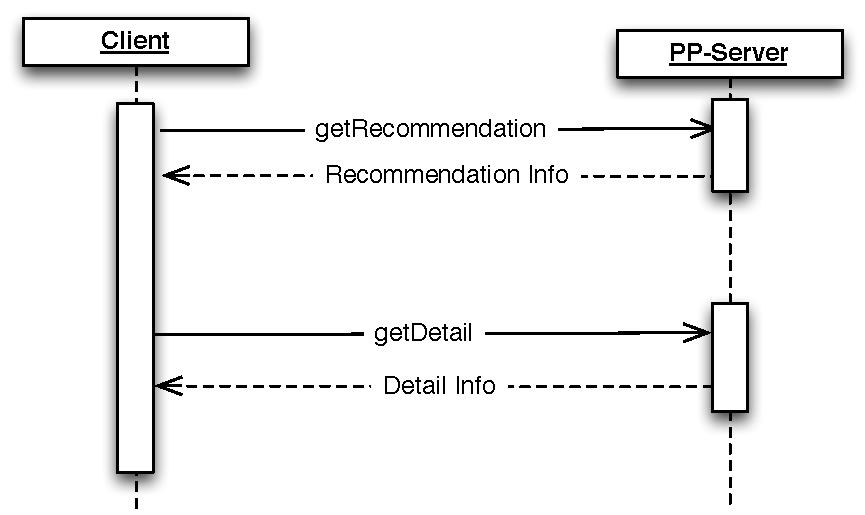
\includegraphics[width=0.75\textwidth]{clientServerComm}
    \caption{Beispiel für Informationsanfrage an den EEXCESS PP--Service}
    \label{fig:clientServerEEXCESS}
\end{figure}

Im ersten Schritt wird eine durch Suchparameter beschriebene
\Verb|/recommend|--Anfrage an der Server gestellt. Die Antwort darauf
besteht aus einem JSON--Objekt. Es enthält, neben den eigentlichen
Ergebnissen der Suchanfrage, auch eine eineindeutige ID zur späteren
Referenzierung der Anfrage. Die zurückgelieferten Ergebnisse bestehen
ihrerseits wieder aus verschiedenen Elementen, unter anderem einem
Titel der das Element näher beschreibt, einer URI die angibt wo das
Objekt gespeichert ist und einer eineindeutigen ID zur Referenzierung
des Objekts. Diese Informationen würden bereits ausreichen, um die einzelnen
Ergebnisse der Suchanfrage aus dem Netz zu laden. Da der Benutzer aber
selber entscheiden soll, ob die angezeigten Zusatzinformationen für
ihn interessant sein könnten, muss er vor der Darstellung eine Auswahl
treffen können. Dies ist anhand des Titels in der Regel nur schwer
möglich!

In einem zweiten, optionalen Schritt kann daher für jedes Ergebnis
einer \Verb|/recommend|--Anfrage eine detaillierte Kurzbeschreibung
vom PP--Server abgerufen werden. Der dafür vorgesehene
\Verb|/getDetails|--Befehl übergibt die ID der Suchanfrage und die
\Verb|documentBadge|--Informationen des ursprünglichen Ergebnisses an
den PP--Server und bekommt, falls bei der Datenquelle hinterlegt, eine
Kurzbeschreibung des Ergebnisses. An Hand dieser Kurzbeschreibung kann
der Anwender dann entscheiden, ob das eigentliche Informations--Objekt
über die zugeordnete URI geladen werden soll oder nicht.

\subsection{\texttt{/recommend}--Anfrage im \SECH--Browser Projekt}
Ein minimales JSON--Objekt für eine \Verb|/recommend|
Anfrage an den PP--Server besteht aus 3~Teilen:
\begin{enumerate}
     \item Den \Verb|origin| Informationen, die den Client näher beschreiben.
     \item Dem \Verb|loggingLevel|, der angibt ob der PP--Server die
    Anfragen aufzeichnen darf oder nicht.
    \item Den \Verb|contextKeywords|, die die eigentlichen
   Suchbegriffe beinhalten.
\end{enumerate}

Über weitere Parameter können die \Verb|/recommend|--Anfrage noch
genauer definiert werden. Im \SECH--Browser werden folgende
Parameter verwendet:
\begin{enumerate}
     \item \Verb|numResults|, um die Anzahl der vom PP-Server
    zurückgegebenen Resultate begrenzen zu können.
     \item Das \Verb|isMainTopic| Attribut der \Verb|contextKeywords|
    Einträge, um bei mehreren Suchparametern eine Priorisierung
    durchführen zu können.
     \item \Verb|interests|, um die Anfragen genauer an die Vorlieben
    des Benutzers anpassen zu können.
     \item \Verb|languages|, um bevorzugt \SECH--Annotations in der
    Muttersprache des Benutzers zu verwenden.
     \item \Verb|timeRange|, um die \SECH--Annotations zeitlich
    eingrenzen zu können.
\end{enumerate}

%Falls vom PP--Server unterstützt, sollen auch folgende Parameter zur
%näheren Beschreibung der Suchanfrage verwendet werden:
%\begin{itemize}
%     \item \Verb|ageRange|
%     \item \Verb|gender|
%     \item \Verb|address|
%\end{itemize}
\part*{Spezifikation}

\part*{Konstruktion}

\part*{zu verteilen}
\chapter*{EEXCESS-Browser}

\section{Funktionalit�ten}

\begin{itemize}
	\item WebView
	\item Back/Forward Button
	\item Lesezeichen
	\item Home-Button
	\item AdressBar
	\item Reload
	\item Men�
\end{itemize}

Mit Hilfe der WebView ist es m�glich, die gew�nschte Webseite anzuzeigen. Befindet man sich auf einer Webseite mit SECH-Tags, so erh�lt man zu diesen zus�tzliche Informationen.

Durch den Back bzw. Forward- Button springt man eine Seite zur�ck bzw. vor. 

In der AdressBar gibt man die URL der gew�nschten Webseite an. Nach einem Klick in die WebView wird die URL gepr�ft und die Seite geladen.

Bei Eingabe eines Suchbegriffs z.B. "Bamberg" wird man auf www.google.de weitergeleitet.

Nach einem Klick auf das Lesezeichensymbol wird die aktuelle Webseite durch Eingabe eines gew�hlten Namens zu den Favoriten hinzugef�gt. 

Durch Klick auf den Home-Button wird man auf die aktuell festgelegte Startseite weitergeleitet.

Durch den Reload-Button ist es m�glich, die aktuelle Webseite neu zu laden.
\chapter{Erstellung des Sechobjects}

\begin{figure}
	\centering
	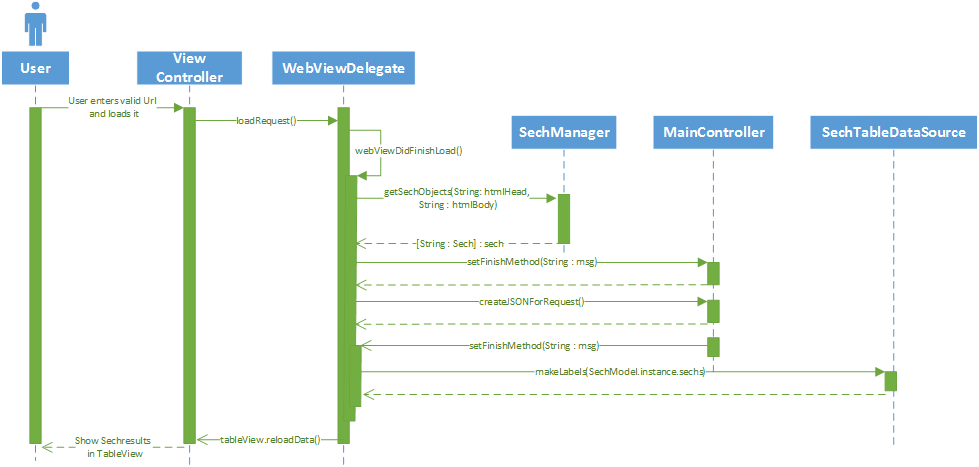
\includegraphics[scale=0.6]{sechobject.png}
	\caption{Ablauf der Erstellung eines \SECH-Objektes}
	\label{fig:SECH-Objekt Erstellung}
\end{figure}

Sobald der User eine gültige URL eingibt und lädt, wird die Laderoutine \Verb|loadRequest()|
angestoßen. Ist die Seite fertig geladen wird in der Delegatemethode \Verb|webViewDidFinishLoad()|
des WebViewDelegates das Auslesen bzw. Laden der \SEARCH-Tags begonnen.

Dem \SEARCH-Manager wird der HTML-Head und Body der eben geladenen Website übergeben und es
werden mit Hilfe des HTMLManagers \SEARCH-Objekte erstellt. Diese \SEARCH-Objekte werden in einem
Dictionary zurückgegeben.

Sobald ein \SECH-Object-Dictionary zurückgegeben wurde, werden die Ergebnisse gerankt und an den SechTableDataSource übergeben. Anschließend wird mit reloadData() die Tabelle der \SECH-Tags im ViewController befüllt.

\begin{document}

\section{Addressbar}
\subsection{Funktionen}
Die Addressbar prüft die Eingaben des Nutzers und schickt diese weiter an die WebView um die Seite anzeigen zu lassen.
Bei Eingabe einer URL wird diese geprüft und an die WebView weitergeschickt um die Webseite anzuzeigen.
Dabei wird die URL nur auf Vollständigkeit geprüft. Falls es dabei zu Fehlern kommt (fehlen von "http://www", "http://" oder "www")
wird die URL ergänzt und erst dann weitergeliefert.
Wenn es sich bei der Eingabe um keine URL handelt, wird die Eingabe an Google weitergeleitet und die Ergebnisse angezeigt.

\subsection{Implementierung}
Die in die Addressbar oder über den HomeButton eingegebene URL wird über die Funktion loadURL() an checkURL weitergeleitet.
Hier wird der String auf Fehler überprüft und der geänderte String zurückgegeben. Danach wird er mit loadRequest() an die
WebView weitergegeben.
\\\\
addressBar/homBTN():\\
Eingabe der URL als String.
\\\\
loadURL():\\
Aufrufe der Verarbeitungsschritte für die URL.
\\\\
checkURL():\\
Aufgeteilt in einzelne Funktinen, welche mit Hilfe von Regulären Ausdrücken die URL nach fehlenden Elementen prüfen.
Falls es Elemtent fehlt wird dieses hinzugefügt. Wenn es sich um keine URL handelt, wird eine URL für die Googlesuche erstellt.
\\\\
validateHTTPWWW():\\
Prüfen nach fehlendem "http://www".
\\
validateHTTP():\\
Prüfen nach fehlendem "http://".
\\
validateWWW():\\
Prüfen nach fehlendem "www".
\\\\
loadRequest:\\
Weitergabe der geprüften und verbesserten URL an die WebView.
\\\\
\begin{figure}
	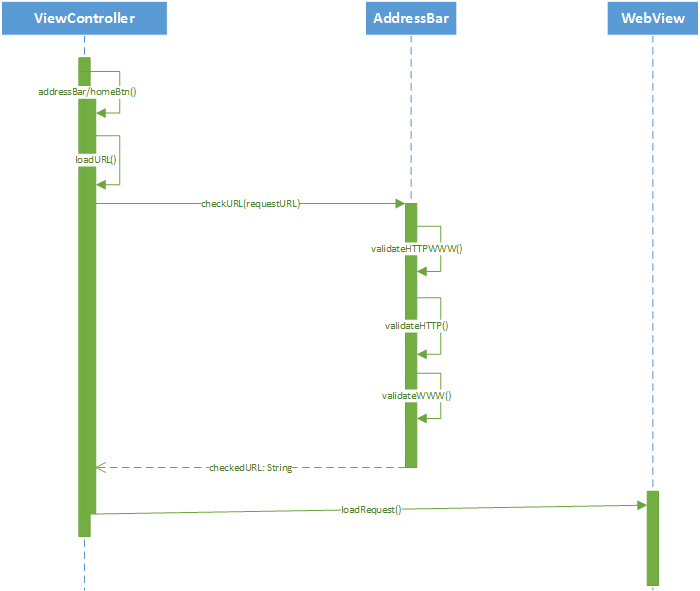
\includegraphics[width=\textwidth]{Pics/AddressCheck.png} 
	\caption{Sequenzdiagramm Adressbar}
	\label{fig:bild}
\end{figure}



\end{document}

%opening
\title{Animation der TableView}
\author{Burak Erol, Philipp Winterholler}

\section{Animation der TableView}

Um eine Übersicht aller gefundenen Sech Tags grafisch darzustellen, wurde ein Label ÃŒber den Sech-Button ergÀnzt, welche die Anzahl der Sech-Tags in einer roten Schrift angibt. Diese Anzahl soll dem Nutzer zeigen, wie viele Sech Tags sich auf der Webseite befinden. Beim Bedienen des Sech Buttons, wird die Sech Tabelle animiert herbei gerufen. Diese Tabelle wird rechts im Browser ein- und ausgefahren. Das WKWebView wird dementsprechend vergrößert oder verkleinert. Bedient man diesen Sech Button, so fährt sich eine Tabelle vom rechten Bildschirm aus und liefert alle Tags in einer TableView zurÃŒck. Die zurÃŒckgelieferten Tags werden in seperaten Zellen auf der TableView abgespeichert, die durch anklicken eine neue Pop-Up Seite, spezifisch zu dem angeklickten Tag, öffnet. Aufgrund der Umstellung der Navigationsleiste wird diese grafische Darstellung der Anzahl an Sech-Tags nicht mehr angezeigt. Die Umstellung der Navigationsleiste war notwendig um die Höhe und Breite des WKWebViews festzulegen, darum ist ein neuer Navigation Controller erzeugt worden, welche die Navigation Bar automatisch mitliefert. In die neue Navigation Bar kann jedoch kein Label hinzugefügt und spezifisch positioniert werden, somit wurde diese Option entfernt.

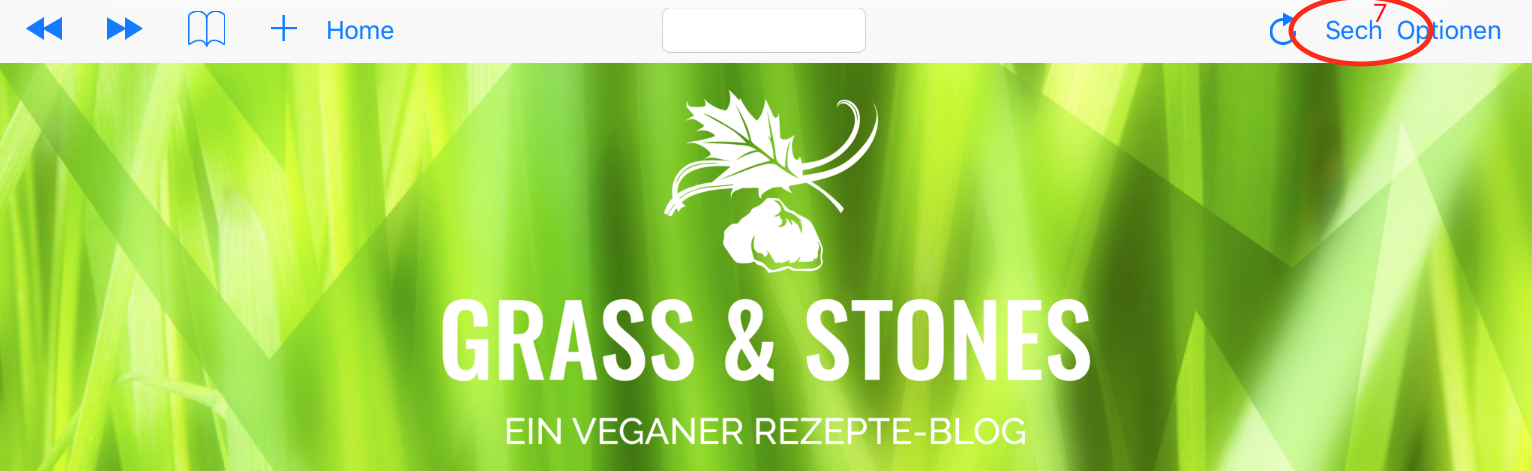
\includegraphics[width=12cm]{Pics/Sech_Anzahl}
\newpage
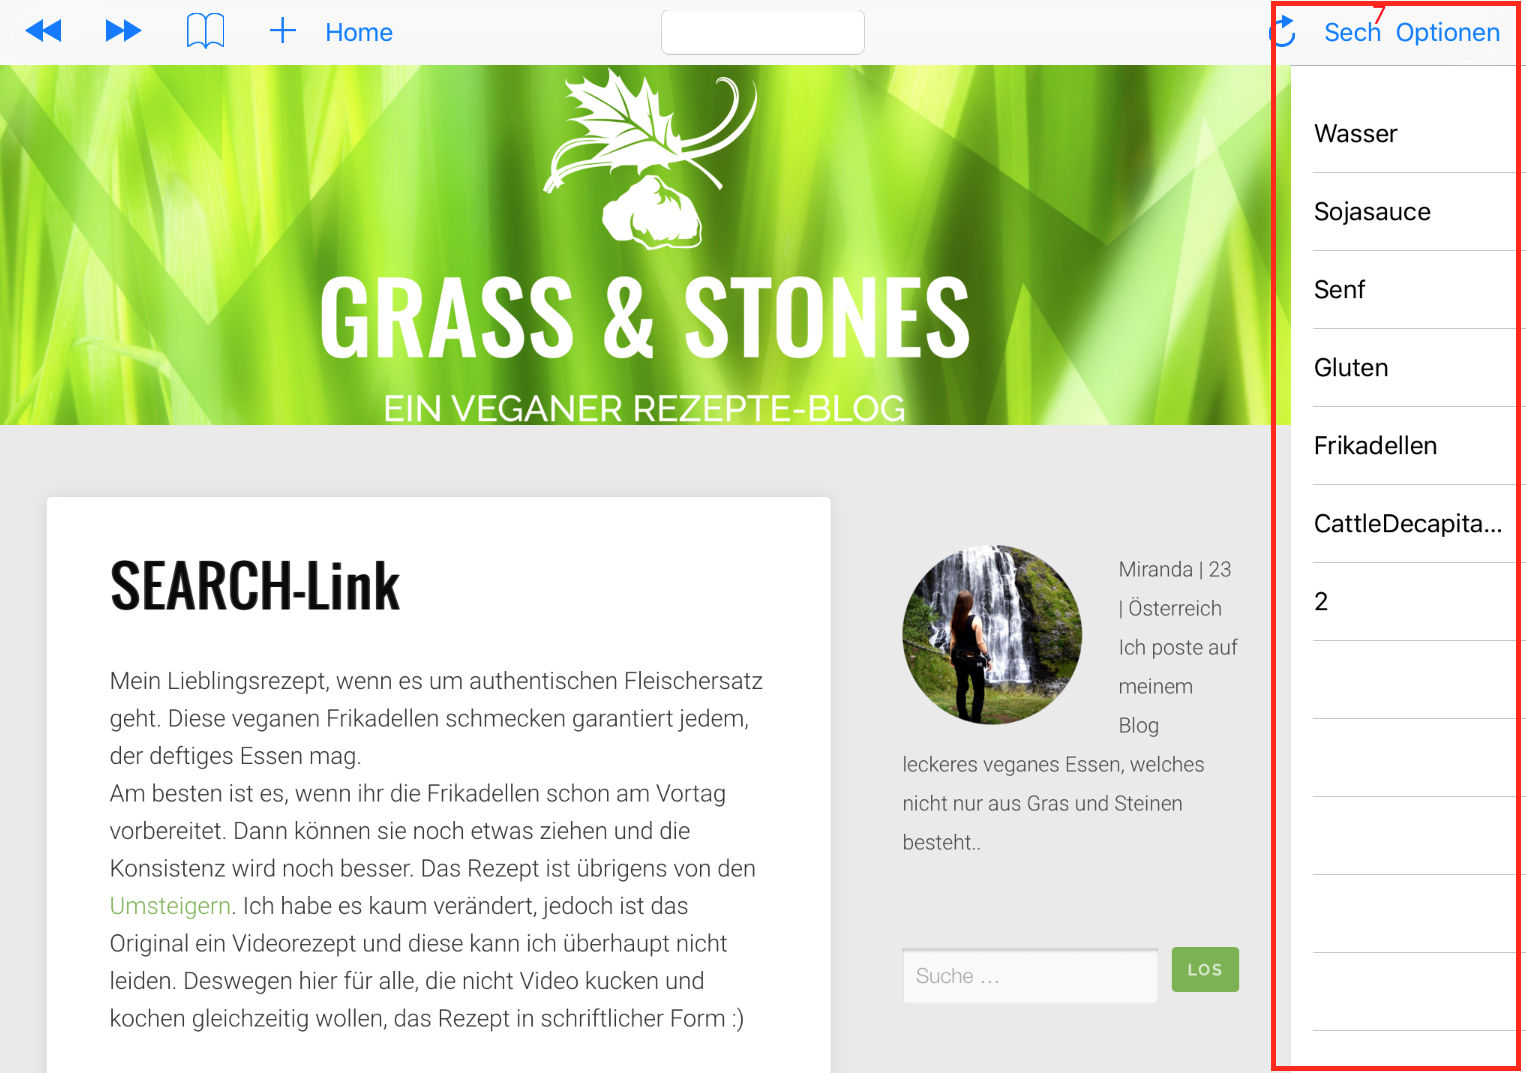
\includegraphics[width=12cm]{Pics/Sech_Tabelle_aufgeklappt}
\newpage
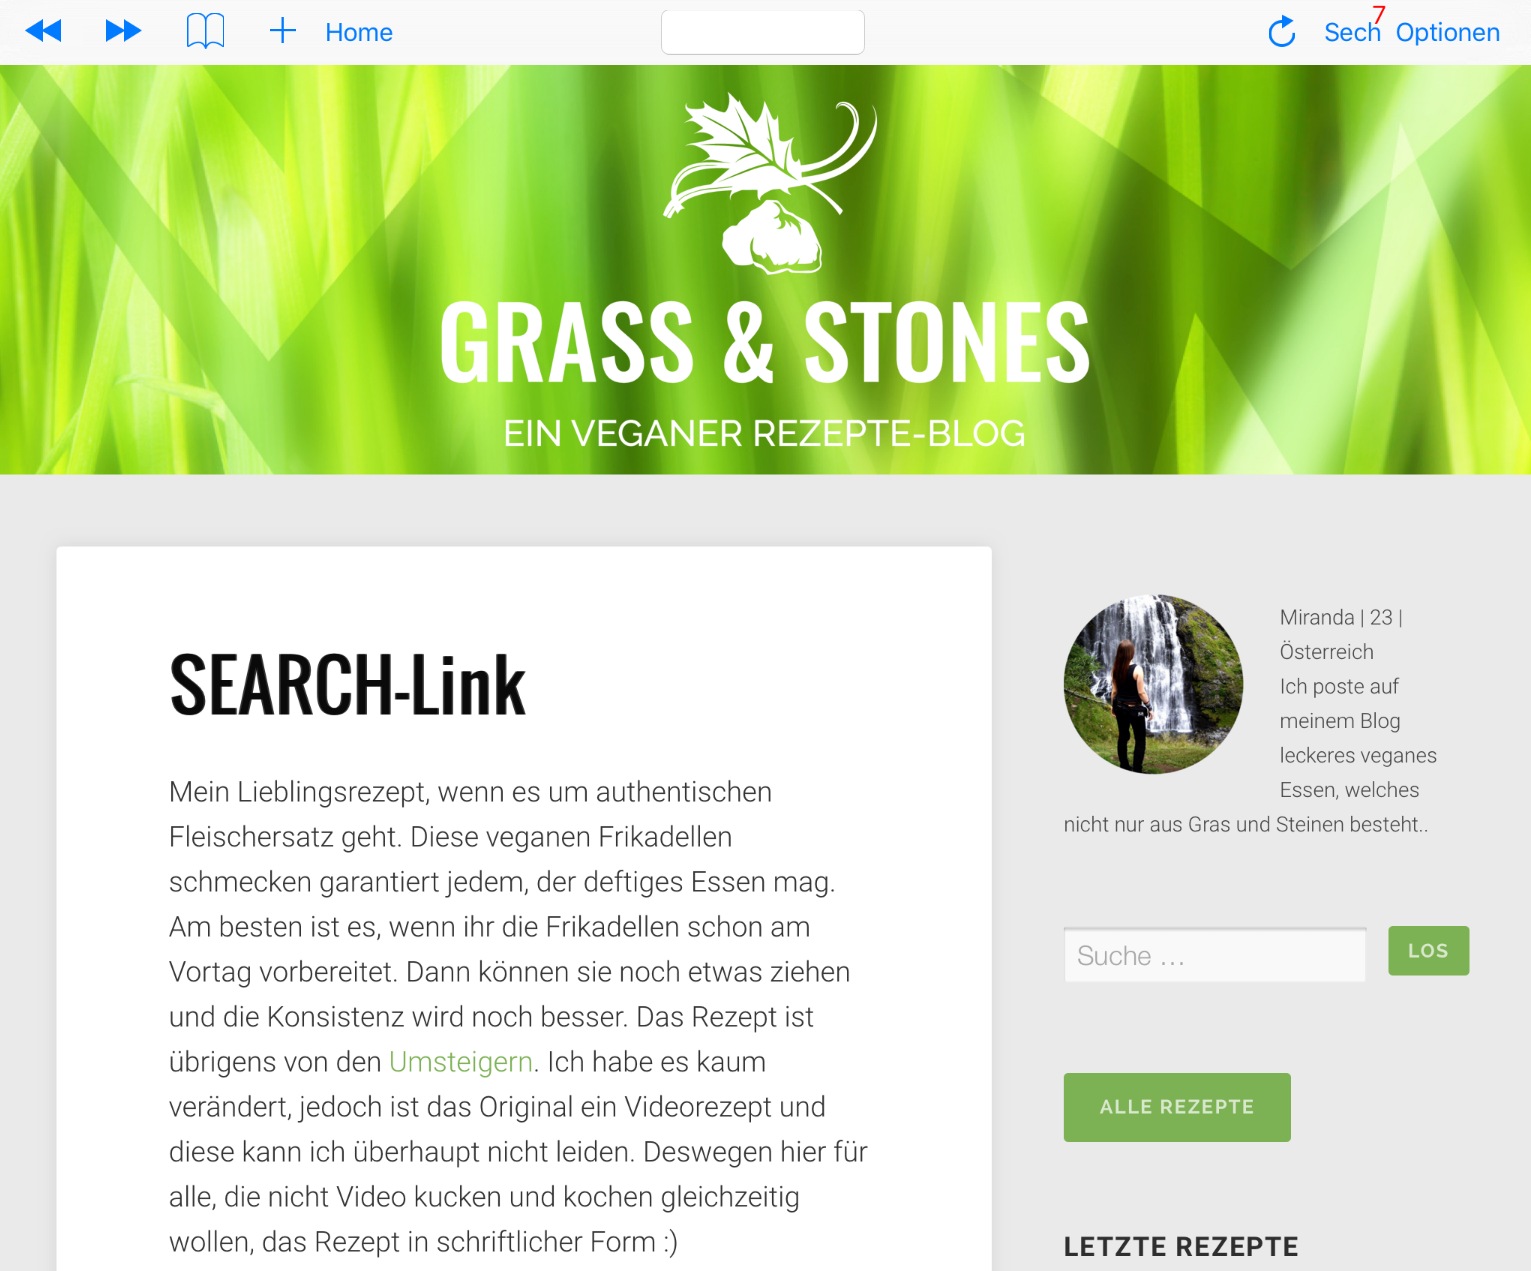
\includegraphics[width=12cm]{Pics/Sech_Tabelle_versteckt}




%opening
\title{Constraints setzen}
\author{Burak Erol, Philipp Winterholler}

\section{Constraints setzen}

Damit die Bedienelemente und das UI vom Browser auf verschiedenen Endgeräten identisch dargestellt wird, müssen Constraints gesetzt werden. Somit wird eine dynamische und bei bestimmten Bedienelementen eine feste Position gesetzt bzw. angepasst. Komplikationen mit den schon vorhandenen Constraints vom Container im Hintergrund waren vorhanden, somit mussten alle Constraints gelöscht und neu erzeugt werden. Nachdem das WKWebView dennoch keine Höhe und Breite vom darunter liegenden Container angenommen hatte (Vermutung: Im main.storyboard nicht verwendete Constraints, die das Layout ungewollt ändern), musste der Navigation Controller gelöscht und erneut integriert werden. Hierzu wurden folgende Schritte beachtet:

- Referenzen der Bedienelemente im main.storyboard und im ViewController löschen 
- Menüleiste samt Buttons im main.storyboard löschen 
- Tabelle/Zellen löschen
- Container im Hintergrund löschen
- Navigation Controller ausklinken und entfernen

Navigation Controller neu erstellen:
- Menüleiste samt Buttons einfügen und feste Constraints setzen
- Container einfügen und feste Constraints setzen
- Tabelle/Zellen einfügen und feste Constraints setzen
- Referenzen neu verlinken und alles wieder in den ViewController integrieren

Nach erfolgreichem absolvieren dieser Schritte wurden im ViewController zwei Contraints erzeugt. Diese dienen für die Zuweisung der Höhe und Breite vom Container auf den darüber liegenden WKWebView, welches programmatisch erzeugt wird. Ändern sich die Constraints vom Container, beispielsweise beim rotieren des Endgerätes, so ändert sich auch Höhe und Breite des WKWebViews.

Ein weiteres Problem stellte die Navigation Bar dar, da diese im nachhinein ergänzt wurde, anstatt sie über einen Navigation Controller zu erzeugen. Das Layout wurde nun neu aufgesetzt und eine vom Navigation Controller erzeugte Navigation Bar verwendet. Gleichzeitig wurde das Problem, in der der Container verschoben wurde und das darüber liegende WKWebView verrutscht ist, gelöst, da diese Constraints sich nun von der Navigation Bar aus orientieren.

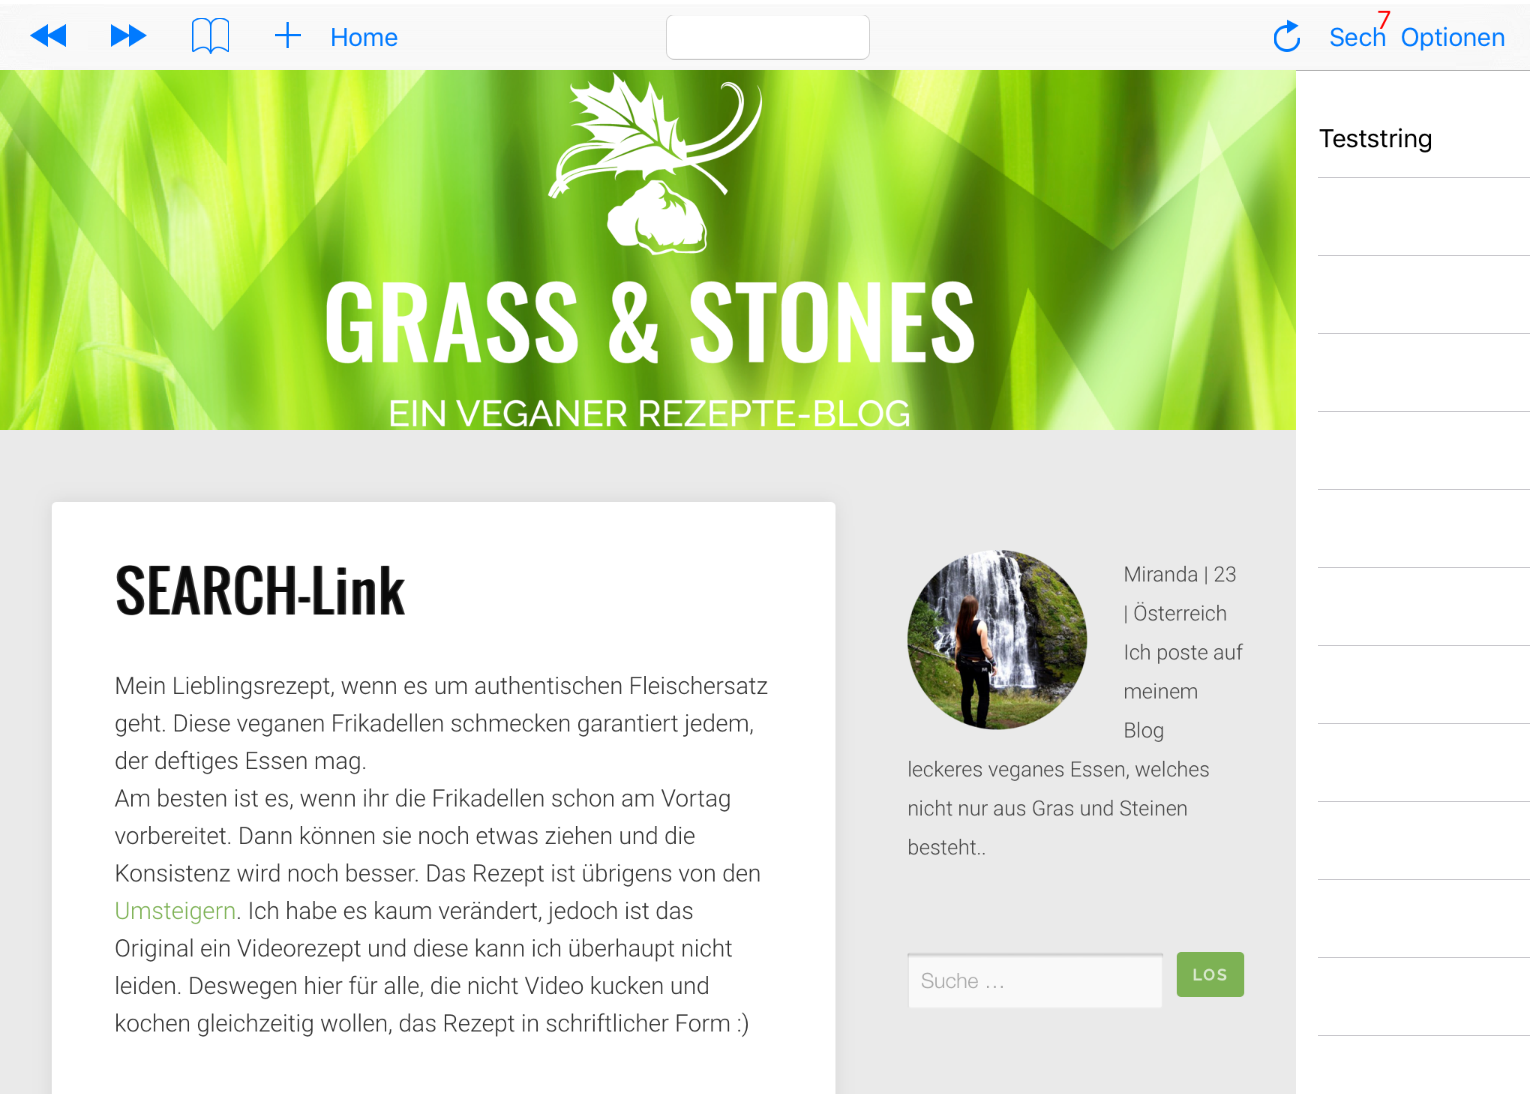
\includegraphics[width=12cm]{Pics/WKWebView_Hochformat}
\newpage
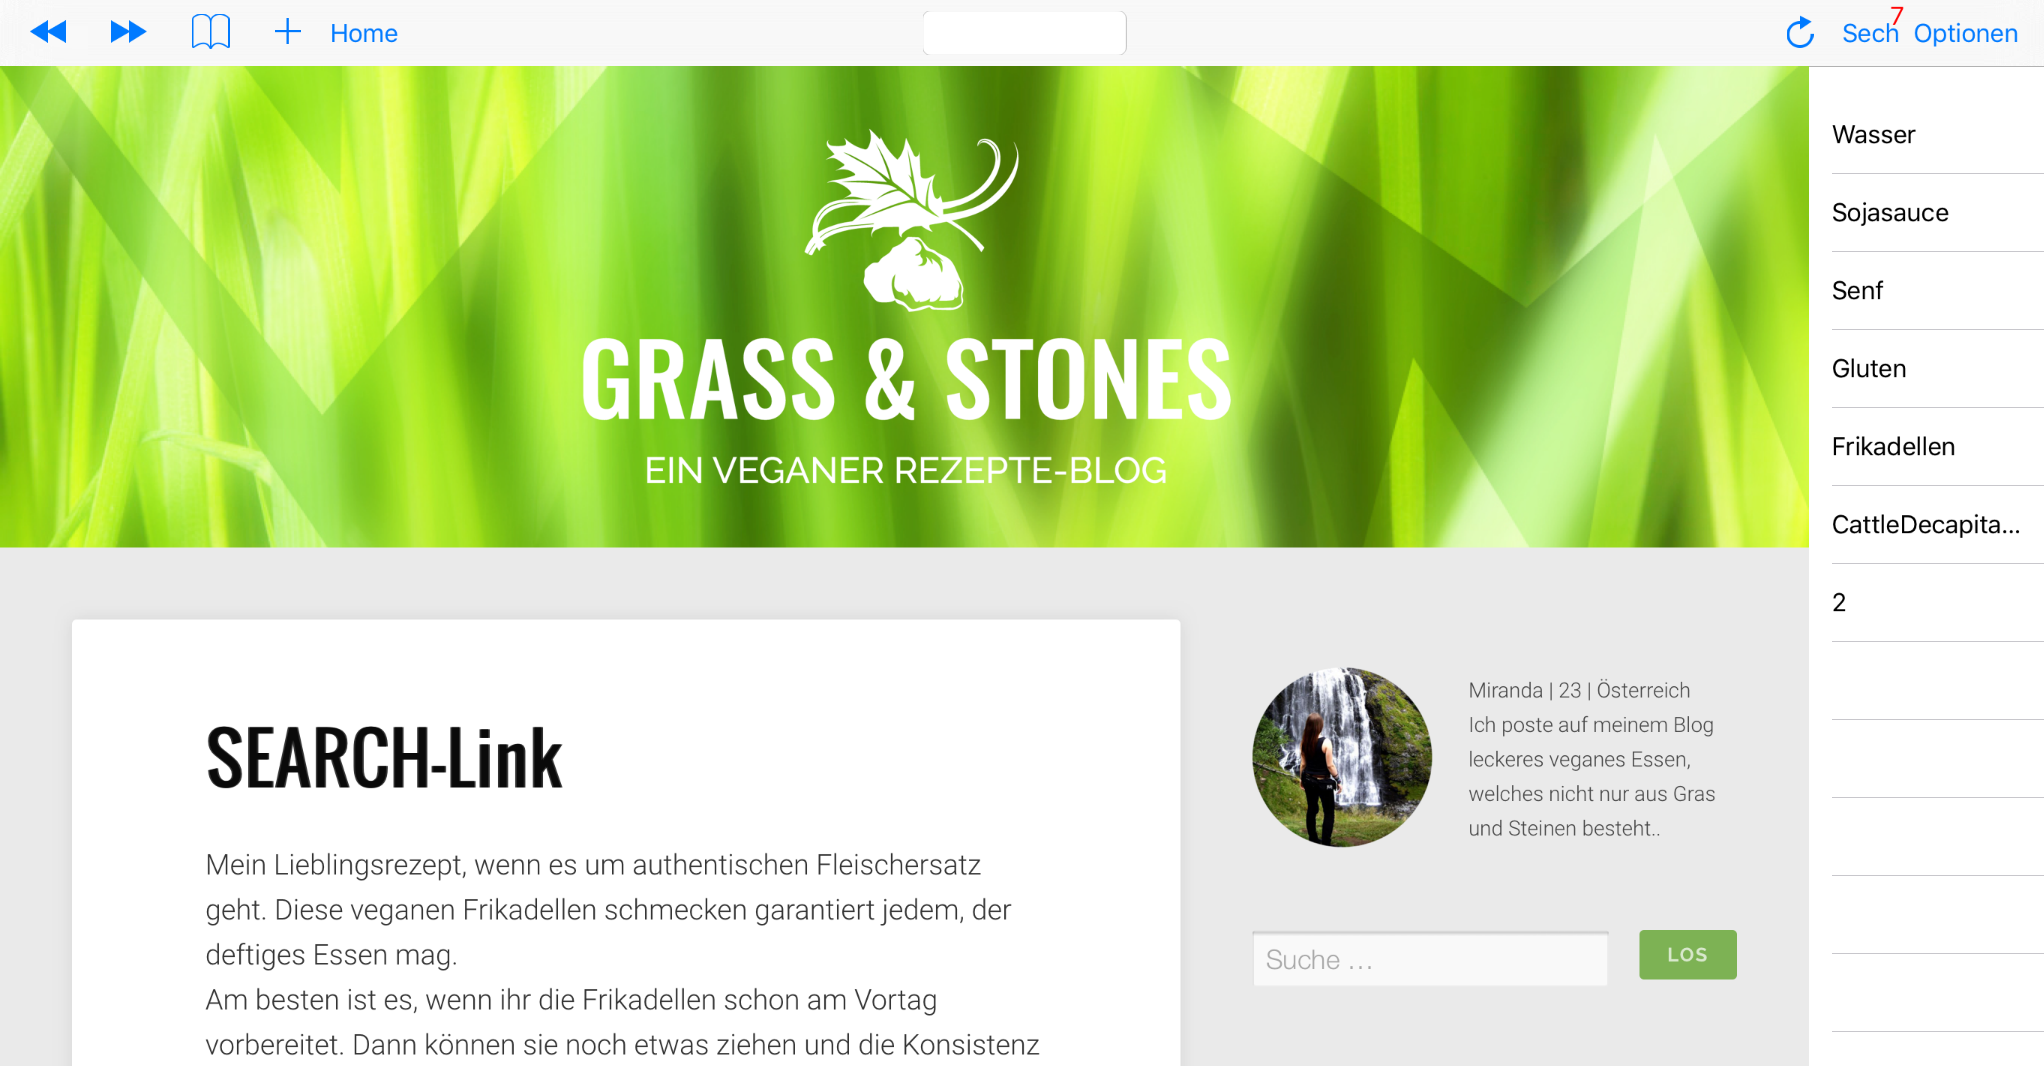
\includegraphics[width=12cm]{Pics/WKWebView_Querformat}




\title{Beschreibung des Prototypen-Content}
\author{apoehlmann}
\date{7.11.2015}

\pdfinfo{%
  /Title    (Beschreibung des Prototypen-Content)
  /Author   (apoehlmann)
  /Creator  (apoehlmann)
  /Keywords (SECH EEXCESS Content Prototyp)
}

\section{Netzwerkverbindungen}

Die Klasse \href{https://github.com/SECH-Tag-EEXCESS-Browser/iOSX-App/blob/master/Team%20Content/Demos/JSON/Sech/Sech/ConnectionManager.swift}{ConnectionManager} ist für das Erstellen einer Verbindung zum Server zuständig. Sie besitzt eine öffentliche Methode ''makeHTTP\_Request''.
 Zusätzlich gibt es eine Klasse \href{https://github.com/SECH-Tag-EEXCESS-Browser/iOSX-App/blob/master/Team%20Content/Demos/JSON/Sech/Sech/ConnectionManager.swift}{PROJECT\_URL} für die URLs, welche im Projekt benötigt werden.

\chapter{Server Anfragen}

\section{Beschreibung}
Der Content-Prototyp ermöglicht es, Anfragen an den Server des  
\href{https://github.com/EEXCESS/eexcess/wiki}{EEXCESS-Projektes} zu schicken.
Der Prototyp unterstützt das \href{https://github.com/EEXCESS/eexcess/wiki/%5B21.09.2015%5D-Request-and-Response-format#pp-query-format}{PP-QF2}
und somit auch das \href{https://github.com/EEXCESS/eexcess/wiki/%5B21.09.2015%5D-Request-and-Response-format#pp-response-format}{PP-RF2}.

\section{Verarbeiten/Aufbauen der Anfragen}
\subsection{Anfrage}
\begin{enumerate}
  \item Auslesen der Suchbegriffe
    \begin{itemize}
      \item Beachten der Trennung der Suchbegriffgruppen
      \item Einfügen in ein Dictionary, als Schlüssel wird der Suchbegriff genommen
      \item Die Schlüssel werden in die ComboBox für das Bearbeiten der Werte eingefügt
    \end{itemize}
  \item Die Suchbegriffe der Parameter werden bearbeitet (isMainTopic und Type) (optional)
  \item Eingabe der Preferenzen (optional)
  \item Abschicken der Anfrage:
    \begin{enumerate}
      \item Suchwörter, Preferenzen und die generierte QueryID werden an den \href{https://github.com/SECH-Tag-EEXCESS-Browser/iOSX-App/blob/master/Team%20Content/Demos/JSON/Sech/Sech/MainController.swift}{MainController} weitergegeben
      \item Übergabe der Werte an den \href{https://github.com/SECH-Tag-EEXCESS-Browser/iOSX-App/blob/master/Team%20Content/Demos/JSON/Sech/Sech/JSONManager.swift}{JSONManager}
      \item Die Schlüssel werden in die ComboBox für das Bearbeiten der Werte eingefügt
      \item Werte werden in das \href{https://github.com/SECH-Tag-EEXCESS-Browser/iOSX-App/blob/master/Team%20Content/Demos/JSON/Sech/Sech/Json.swift}{JSONObject} eingefügt und zurückgegeben
      \item JSONObject wird über den MainController an den \href{https://github.com/SECH-Tag-EEXCESS-Browser/iOSX-App/blob/master/Team%20Content/Demos/JSON/Sech/Sech/ConnectionManager.swift}{ConnectionManager} weitergegeben
      \item Der ConnectionManager verschickt die Daten an den Server
    \end{enumerate}
  \item Die Antwort vom Server wird im \href{https://github.com/SECH-Tag-EEXCESS-Browser/iOSX-App/blob/master/Team%20Content/Demos/JSON/Sech/Sech/ViewController.swift}{ViewController:53} entgegen genommen und dargestellt
  \item Speichert JSON in das Dictionary \glqq mapOfJSONs \grqq\ in der Klasse \glqq MainController\grqq\ 
  \item Fügt die DocumentBadges in die die ComboBox für die DetailAnfrage
\end{enumerate}
\pagebreak
\subsection{DetailAnfrage}
    \begin{enumerate}
      \item Auswahl des DocumentBag oder der \glqq take all\grqq Option
      \item Betätigen des \glqq Search Details\grqq\ -Buttons
	\begin{enumerate}
	  \item Übergibt den DocumentBag/DocumentBags an den JSONManager über den MainController
	  \item JSONObject wird erzeugt und zurückgegeben
	  \item DetailAnfrage wird an den Server übermittelt
	\end{enumerate}
      \item Antwort wird vom ViewController entgegengenommen und im TextFeld dargestellt
    \end{enumerate}

\pagebreak
\section{JSON Objekt}

Der JSON wird in der Klasse \href{https://github.com/SECH-Tag-EEXCESS-Browser/iOSX-App/blob/master/Team%20Content/Demos/JSON/Sech/Sech/Json.swift}{JSONObject} 
gehalten. Ein Dictionary in der Klasse speichert alle Schlüssel/Wert-Paare des JSONObjects.
Es gibt drei Varianten für das Erstellen eines Objekts der Klasse JSONObject:
\begin{itemize}
\item ohne Übergabewert
\item mit einem Dictionary
\item mit einem NSData-Objekt, welches ein Dictionary enthält
\end{itemize}

Die Klasse JSONObject besitzt verschiedene Methoden:
\begin{itemize}
\item Auslesen von Werten (spezialisiert auf bestimmte Datentypen)
\item Einer found()-Methode zum Überprüfen, ob der Schlüssel vorhanden ist
\item Zum Erweitern des JSONs mit Werten
\item Convert-Methoden für das Umwandeln von JSONObject in String und NSData
\end{itemize}

Die Klasse JSONObject kann ohne großen Aufwand um weitere Methoden ergänzt werden, wie zum Beispiel um eine Methode, getImage(key:String) zu erweitern.

\section{Prototyp UI}
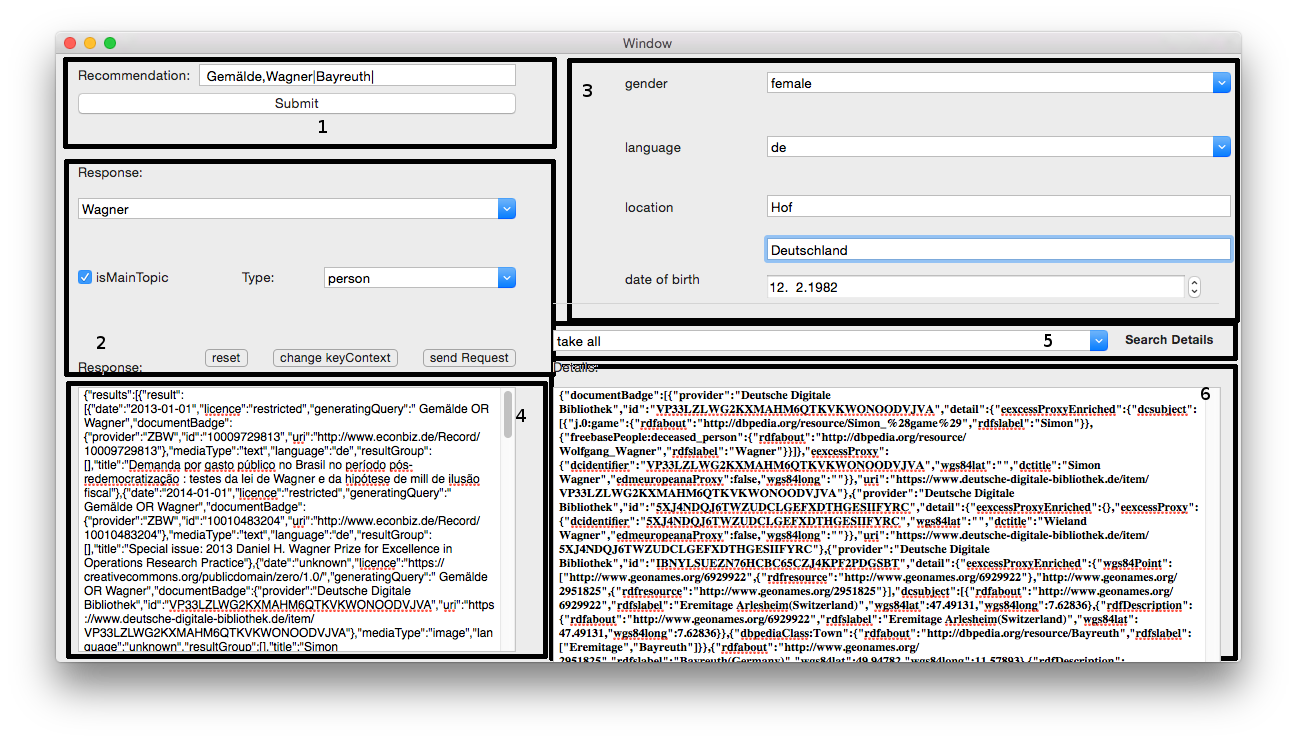
\includegraphics[scale=0.35]{ContentPrototyp2.png}
\begin{enumerate}
\item Eingabe der Suchbegriffe. Mit \glqq ,\grqq\ werden die Begriffe getrennt und mit \glqq |\grqq\ werden die Suchbegriffgruppen getrennt
\item Hier können den Suchbegriffen noch Eigenschaften hinzugefügt werden. Nach jeder Änderung muss der \glqq change keyContext\grqq\ -Button gedrückt werden. Mit dem Button \glqq send Request\grqq\ wird die Anfrage verschickt. Der Button \glqq reset\grqq\ besitzt keine Funktion.
\item In diesem Bereich können zusätzliche Informationen für die Anfrage angegeben werden.
\item Anzeige der Antwort vom Server
\item Auswahlmöglichkeiten für die Detailanfrage und der \glqq Search Details\grqq\ -Button
\item Anzeige der DetailAntwort vom Server
\end{enumerate}


\documentclass[a4paper,12pt]{article}
\usepackage[utf8]{inputenc}
\usepackage[german, ngerman]{babel}
\usepackage{graphicx}
\usepackage[figurename=Bild]{caption}
\usepackage{inputenc}
\usepackage{geometry}


%opening
\title{Entwicklung des Layouts des Browsers}
\author{Burak Erol, Andreas Netsch, Philipp Winterholler}

\begin{document}

\section{Entwicklung des Layouts des Browsers}

Das Layout des Browsers besteht aus folgenden Elementen:

- Navigation Controller
- Navigation Bar
	- Back/Forward Button
	- Lesezeichen Button
	- Lesezeichen hinzuf�gen Button
	- Home Button
	- AddressBar
	- Reload Button
	- Sech Button
	- Optionen Button
- Container
- WKWebView

Die oben aufgelisteten Elemente stellen das komplette Layout des Browser dar. Der Navigation Controller dient in diesem dazu, dem Browser einen automatisch generierten Navigation Bar hinzuzuf�gen, welche im oberen Bildschirm fest verankert ist und eine nicht ver�nderbare H�he und Breite liefert. Diese Navigation Bar besitzt einen Back Button, um auf einer Seite zur�ck zu springen und einen Forward Button, um eine Seite vor zu bl�ttern. Bedient man den Lesezeichen Button so �ffnet sich eine TableView mit aller gespeicherten Seiten chronologisch absteigend. Will der Nutzer die Liste um ein weiteres Element erg�nzen, so muss er den Plus Button bedienen, so �ffnet sich ein Pop Up Fenster, der den Link der aktuell besuchten Seite automatisch �bernimmt und der Nutzer diesem jediglich nur noch einen Titel vergeben und abspeichern muss. Mit dem Home Button gelangt der Nutzer zu seiner definierten Startseite. Die AddressBar dient f�r die Eingabe eines Web Links der durch best�tigen zu der eingegeben Seite gelangt. Um die aktuelle Seite neu zu laden, muss der Reload Button bedient werden und um alle Sech Tags auf der aktuellen Seite anzuzeigen, bedient der Nutzer den Sech Button. Ist der Sech Button angeklickt worden, so klappt sich von der rechten Bildschirmseite eine TableView mit allen Sech Tags auf und bietet dem Nutzer eine �bersicht dieser. Wird eines der Sech Tags in dieser TableView angeklickt, so �ffnet sich ebenfalls ein PopUp Fenster zu diesem Tag, der weitere Informationen zur�ck liefert. Um die Sech Tag Tabelle wieder einzuklappen wird ein weiteres Klicken auf den Sech Button ben�tigt und diese f�hrt sich ein. Durch einen Klick auf den Optionen Button �ffnet sich auch hier ein Pop Up Fenster der benutzerspezifische Informationen mitliefert und �bersichtlich darstellt. Um den WKWebView eine dynamische H�he und Breite programmatisch zu �bergeben wurde ein Container eine Schicht unter diesem mit festen Constraints �bergeben. Diese Constraints passen sich zu den benachbarten Elementen an und das WKWebView �bernimmt die Constraints dieses Containers. Dreht man das Endger�t beispielsweise vom Hochformat in den Querformat, �ndern sich H�he und Breite des Containers und diese werden vom WKWebView �bernommen.

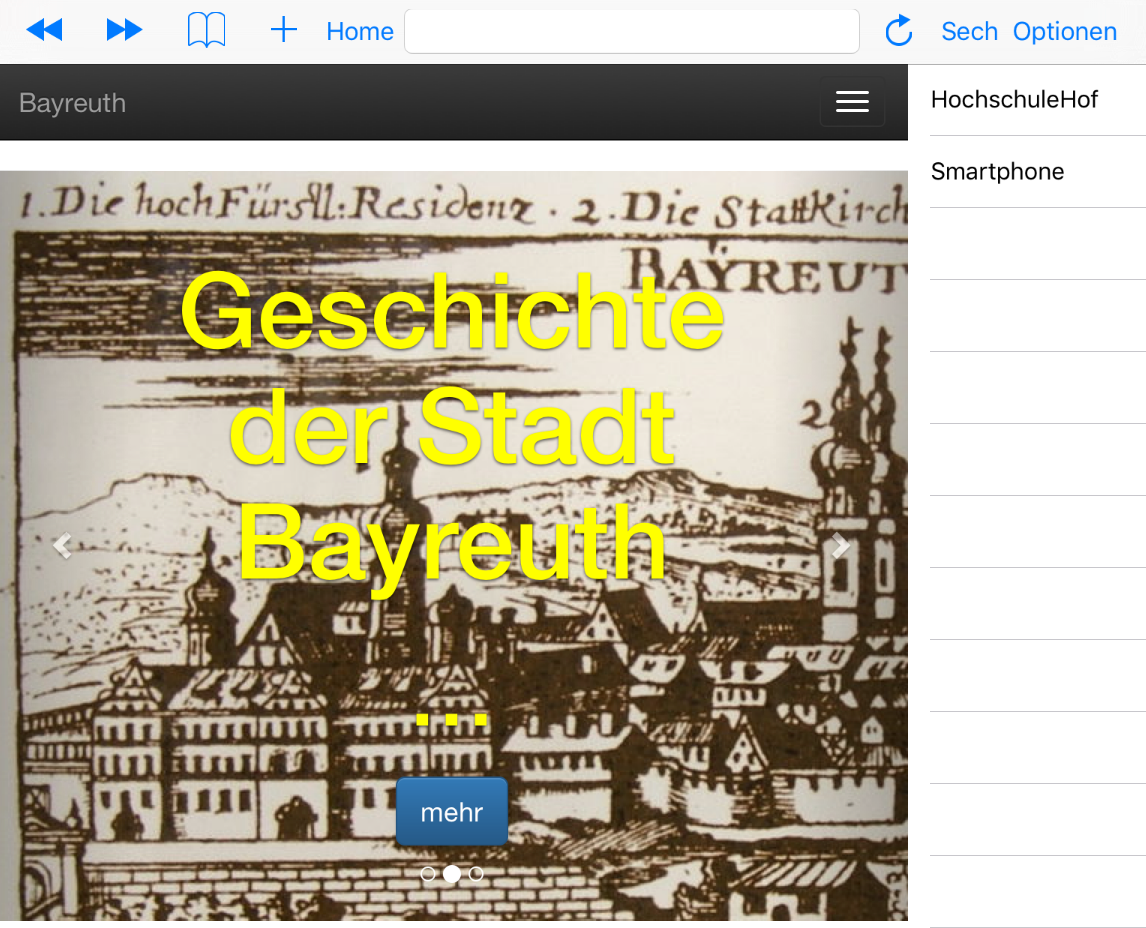
\includegraphics[width=12cm]{Pics/Browser_Hochformat}

\end{document}


%opening
\title{Konstruktion Ranking}
\author{Lothar Mödl}

\chapter{Ranking}
\section{Sequenzdiagramm}

\begin{figure}[h]
	\centering
	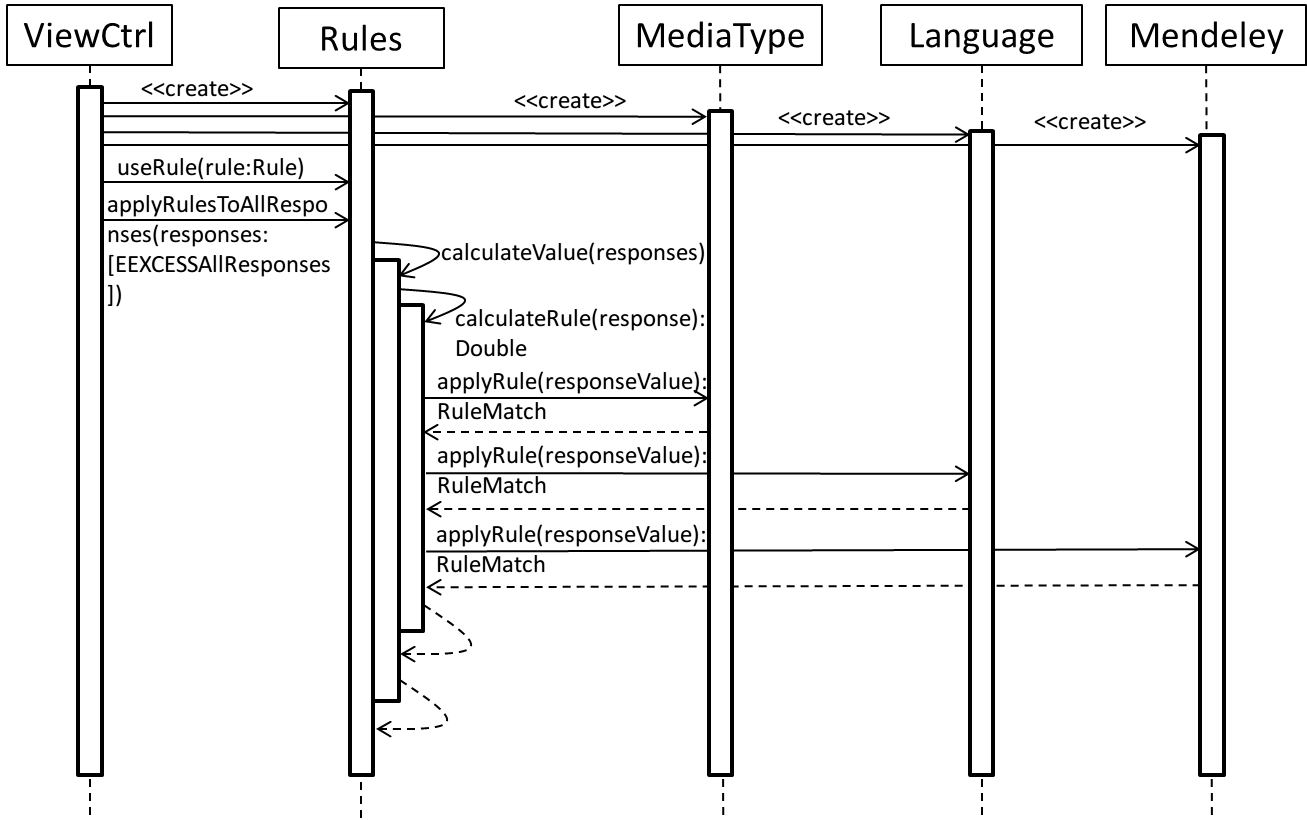
\includegraphics[width=12cm]{Sequenzdiagramm_Ranking}
	\caption{Sequenzdiagramm des Rankings}
	\label{fig:Ranking Sequenzdiagramm}
\end{figure}

Dieses Sequenzdiagramm zeigt einen exemplarischen Durchlauf des Rankings der Vorschläge für den Benutzer. Nachdem die Daten aus dem Internet abgerufen wurden und an den ViewController (Team UI) übergeben wurden folgt die Sortierung der Ergebnisse nach den Interessen des Nutzers. Es existieren eine Reihe an verschiedenen Regeln, die angewendet werden können. Die Anzahl an Regeln kann variieren. Welche Regeln angewendet werden, wird vom ViewController festgelegt mit Hilfe der Methode „useRule(rule:Rule)“. Nachdem die Regeln, die angewendet werden sollen, festgelegt wurden, müssen diese angewendet werden. Dies geschieht mit der Methode „applyRulesToAllResponses(responses:[EEXCESSAlllResponses])“. Als Argument müssen alle zuvor erhaltenen Ergebnisse mit übergeben werden. Die Klasse Rules übernimmt im Anschluss die Berechnungen, die für das Ranking der Ergebnisse notwendig sind. Die Methode „calculateValue(responses)“ berechnet in Verbindung mit der Methode „calculateRule(response): Double“ einen Durchschnittswert für jede einzelne Antwort für jeden einzelnen \SEARCH-Tag, nachdem jede Regel angewendet wurde. Eine Regeln wird durch den Aufruf der Methode „applyRule(responseValue): RuleMatch“ angewandt, welche jede Regel besitzt und liefert den Wert 0 oder 1 zurück. Dieser bedeutet, ob die Regel auf die Interessen des Nutzers zutrifft oder nicht. Zum Abschluss des Rankings werden die einzelnen Ergebnisse entsprechend nach dem zuvor errechneten Durchschnittswert sortiert. Im Anschluss erhält das Team UI die sortierten Werte zurück und kann sie dem Nutzer darstellen. 

\section{Klassendiagramm}

\begin{figure}[h]
	\centering
	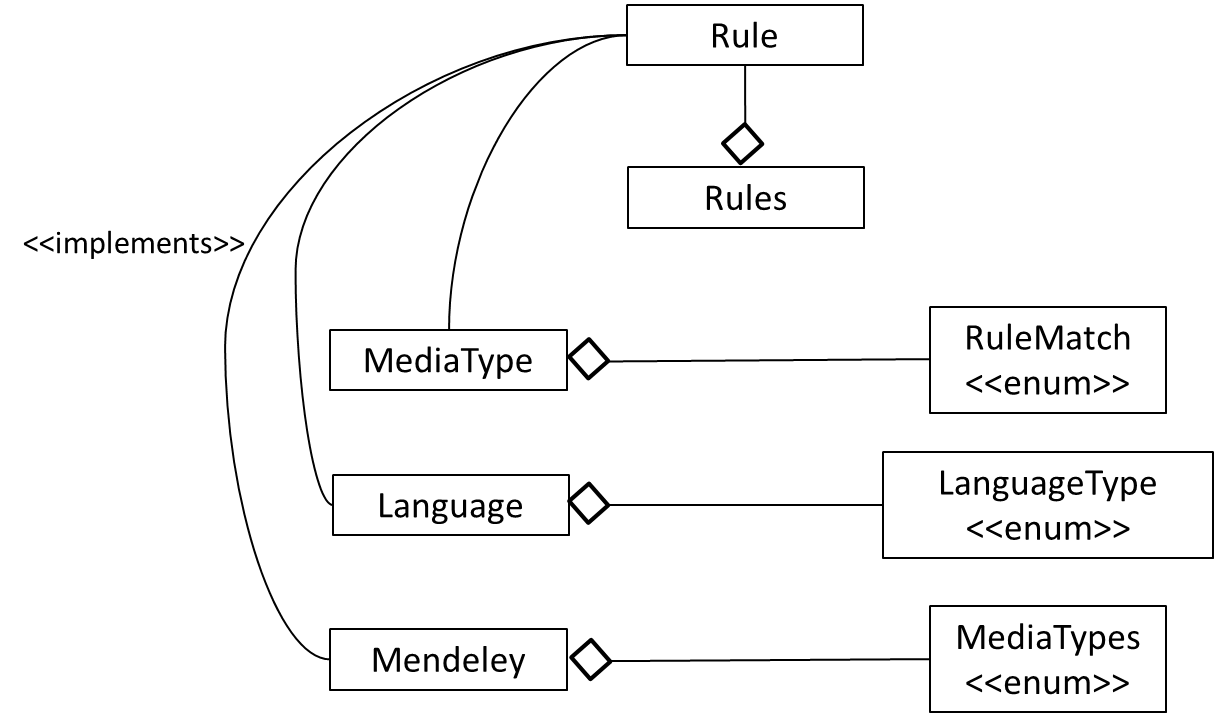
\includegraphics[width=12cm]{Klassendiagramm_Ranking}
	\caption{Klassendiagramm des Rankings}
	\label{fig:Ranking Klassendiagramm}
\end{figure}

\section{Abruf der Daten vom Server Sequenzdiagramm}

Dieses Sequenzdiagramm zeigt einen exemplarischen Ablauf zum Abrufen der Daten vom Server. Zuerst wird eine Instanz des TaskControllers erzeugt. Dieser stellt die Schnittstelle zum View zur Verfügung. Er empfängt und sendet Daten von bzw. an den View. Die Methode „getRecommendations([SEARCHModel], setRecommendations:(String, [Response]))“ bildet die Schnittstelle, bei der die einzelnen, aus der HTML Seite ausgelesenen, SEARCH-Tags in Form von SEARCHModels übergeben werden, sowie die Methode „setRecommendations(String, [Responses])“, die für die Rückgabe der heruntergeladen Ergebnisse zuständig ist. Im Anschluss wird eine Instanz des JSONConnectionControllers sowie des EEXCESSRecommendationJSONControllers erzeugt. Der JSONConnectionCtrl ist für den Aufbau der Verbindung zum Server zuständig. Beim Erzeugen es EEXCESSRecommendationJSONControllers werden die SEARCHModels in einen JSON String konvertiert. Mit Hilfe der Methode „post(AnyObject, String, postCompleted(Bool, NSData))“ wird zuvor erzeugte JSON String an den Server gesendet. Nach Erhalt der Daten wird die Methode postCompleted(Bool, NSData) mit diesen heruntergeladenen Daten aufgerufen. Innerhalb von 
postCompleted(...) wird wiederum eine Instanz des EEXCESSRecommendationControllers erzeugt, welcher die JSON Daten parst und in die interne Struktur der App überführt. Hierfür wird für jede einzelne Antwort eines \SEARCH-Tags eine Instanz von EEXCESSSingleResponse erzeugt. Alle Antworten, die zu einem \SEARCH-Tag gehören, werden in einer neuen Instanz von EEXCESSAllResponses gespeichert.  Das komplette Array von allen EEXCESSAllResponses wird an den TaskCtrl zurückgegeben. Dieses Array wird mit der zu Beginn erhaltenen Methode „setRecommendations(String, [EEXCESSAllResponses])“ an den View zurückgegeben, welcher die Ergebnisse dann darstellt. 

\begin{figure}[h]
	\centering
	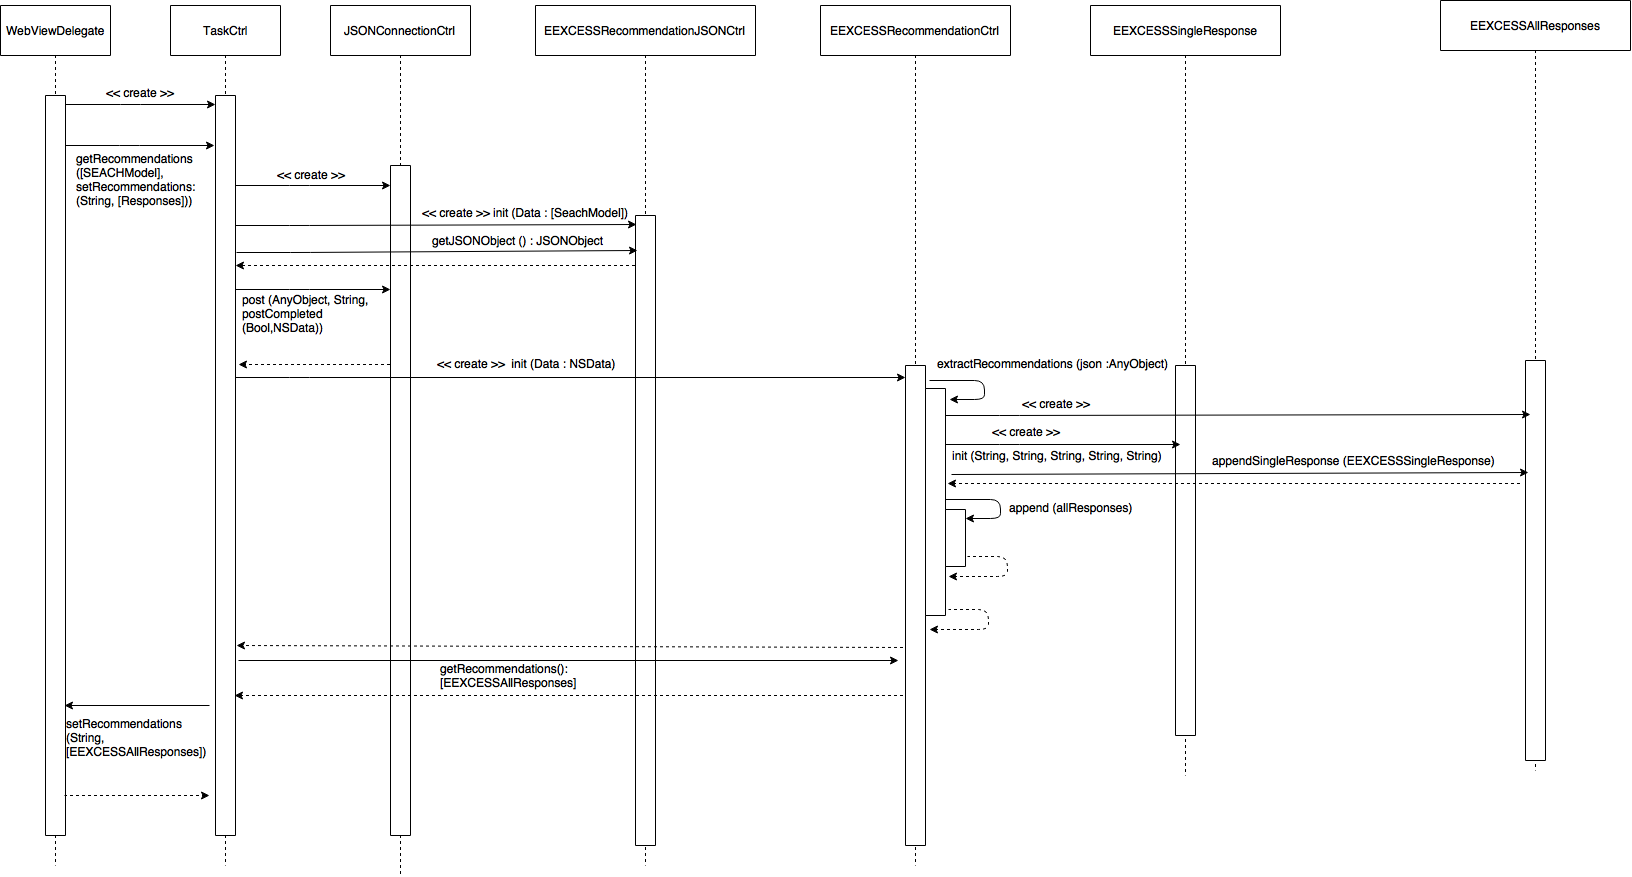
\includegraphics[width=12cm]{Sequenzdiagramm_Anfragen}
	\caption{Sequenzdiagramm einer Serveranfrage}
	\label{fig:Anfrage Sequenzdiagramm}
\end{figure}

\section{Abruf der Daten vom Server Klassendiagramm}

\begin{figure}[h]
	\centering
	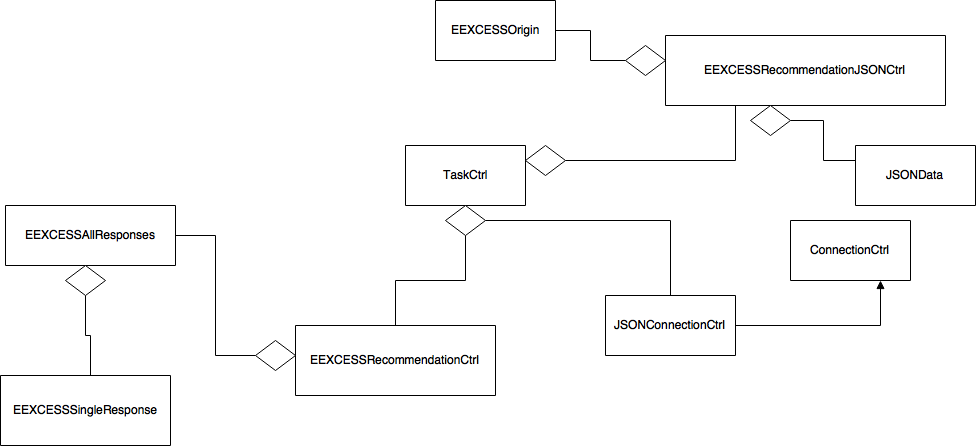
\includegraphics[width=12cm]{Klassendiagramm_Anfrage}
	\caption{Klassendiagramm einer Serveranfrage}
	\label{fig:Anfrage Klassendiagramm}
\end{figure}

\begin{document}
\maketitle
\tableofcontents
\pagebreak

\section{Lesezeichen hinzufügen}
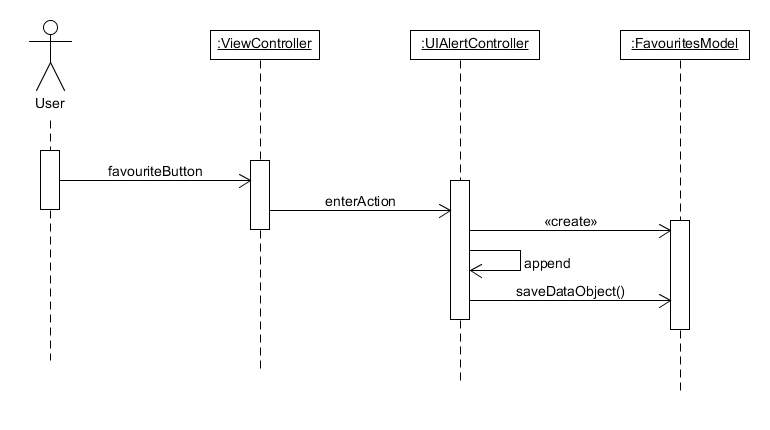
\includegraphics[scale=0.5]{sequAddFavourites.png}
Nachdem der User auf den Plusbutton zum Hinzufügen eines neuen Lesezeichens klickt, wird im ViewController die IBAction des Buttons aufgerufen. Hier wird die enterAction des UIAlertControllers aufgerufen. Nun kann der Nutzer den gewünschten Titel des Lesezeichens eingeben. Die URL wird automatisch übernommen. Nachdem man auf Enter zum Bestätigen klickt, wird ein neues Objekt des FavouriteModels erzeugt. Anschließend wird das erstellte Lesezeichen in das Model geschrieben und persistent gespeichert.
\pagebreak

\section{Lesezeichen bearbeiten}
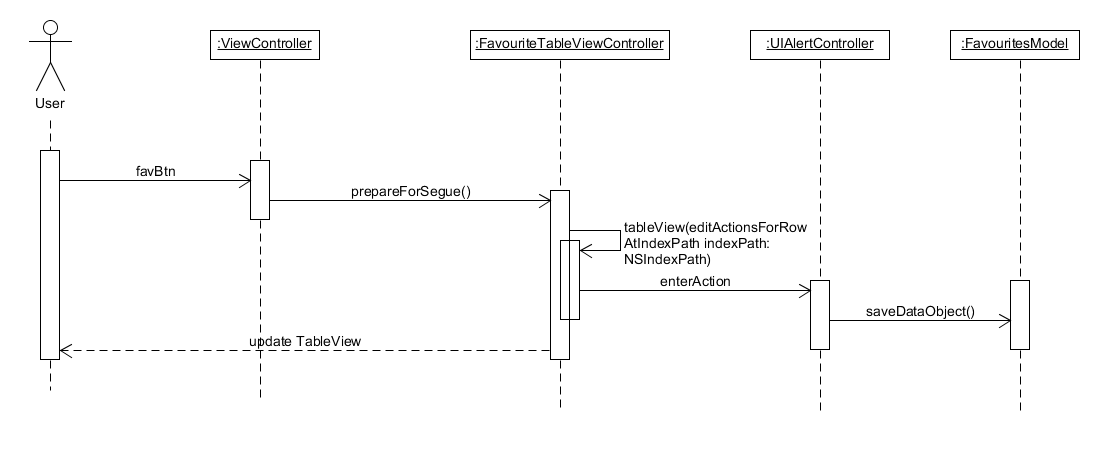
\includegraphics[scale=0.40]{sequEditFavourites.png}
Nachdem der User auf das Lesezeichensymbol zum Anzeigen der gespeicherten Lesezeichen klickt, wird im ViewController die prepareForSegue-Methode aufgerufen. Nun wird der FavouriteTableViewController geladen. Hier wird die Methode editActionsForRowAtIndexPath indexPath: NSIndexPath) aufgerufen. Nachdem man den entsprechenden Eintrag in der TableView auswählt, öffnet sich ein AlertFenster. Hier ist es möglich, den Titel zu ändern. Nach dem Bestätigen wird dies persistent gespeichert und die TableView aktualisiert.
\pagebreak

\section{Lesezeichen anzeigen}
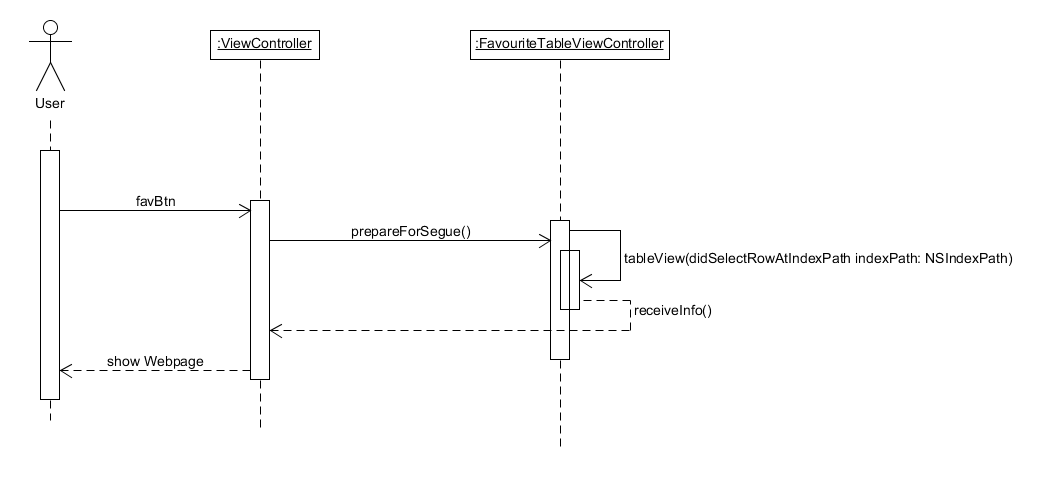
\includegraphics[scale=0.45]{sequShowFavourites.png}
Nachdem der User auf das Lesezeichensymbol zum Anzeigen der gespeicherten Lesezeichen klickt, wird im ViewController die prepareForSegue-Methode aufgerufen. Nun wird der FavouriteTableViewController geladen. Hier wird die Methode tableView(didSelectRowAtIndexPath indexPath: NSIndexPath) augerufen. Hier wird überprüft, ob der Nutzer auf eine Zelle der TableView geklickt hat. Sobald man auf eine Zelle klickt, wird die entsprechende URL im FavouriteModel gespeichert und die Delegate-Methode receiveInfo() im ViewController aufgerufen. Dort wird die Methode loadURL mit der entsprechenden URL aufgerufen. Anschließend gelangt der Nutzer zum ViewController und die URL wird in der WebView angezeigt.
\pagebreak

\section{Lesezeichen löschen}
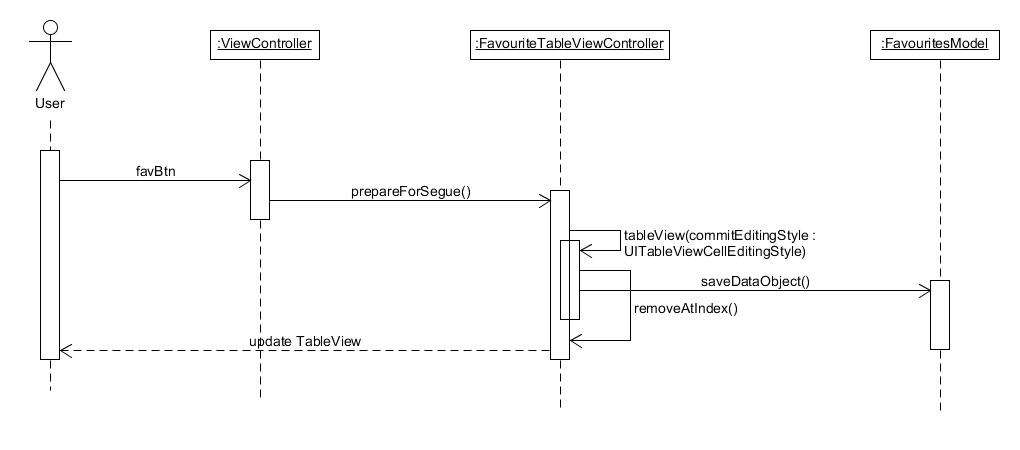
\includegraphics[scale=0.45]{sequDeleteFavourites.png}
Nachdem der User auf das Lesezeichensymbol zum Anzeigen der gespeicherten Lesezeichen klickt, wird im ViewController die prepareForSegue-Methode aufgerufen. Nun wird der FavouriteTableViewController geladen. Hier wird die Methode editActionsForRowAtIndexPath indexPath: NSIndexPath) aufgerufen. Hier wird der ausgewählte Eintrag gelöscht. Dies wird persistent gespeichert und die TableView aktualisiert.
\pagebreak

\end{document}
\documentclass[a4paper,10pt]{article}
\usepackage[utf8]{inputenc}


\begin{document}
\chapter{Bestimmung der Linzenzen der erweiternden Daten}
Für einige Benutzer des EEXCESS-Browsers ist es für die weitere Verwendung der erweiternden Daten notwendig zu wissen, welchen Lizenzen diese unterliegen. Hierfür wird die Methode „getLicenceType(licenseURL: String) ->LicenceType“ verwendet. Diese Methode erhält als Eingabeparameter die URL der Lizenz des jeweiligen Objekts als String, welche vom EEXCESS-Server zurückgeliefert wird, und liefert einen Enum-Type zurück. Als Enum-Type sind folgende verfügbar:
\begin{itemize}
\item CreativeCommon
\item Restricted
\item Europeana
\item Other
\end{itemize}

Diese Lizenzen geben an, ob die Daten ohne Weiteres für andere Zwecke verwendet werden dürfen oder irgendwelchen Lizenzbestimmungen unterliegen.
\end{document}


\chapter{Einstellungsmöglichkeiten}

Der Nutzer hat die Möglichkeit bestimmte Einstellungen vorzunehmen, welche die Ergebnisse der Suchanfragen beeinflussen.   

Folgende Einstellungen können getätigt werden:

\begin{itemize}
	\item Geschlecht des Nutzers (männlich, weiblich)
	\item vom Nutzer bevorzugte Sprache (deutsch, englisch)
	\item Stadt
	\item Land
	\item Geburtsdatum des Nutzers
\end{itemize}


Nachdem der Nutzer alle Einstellungen getätigt hat, werden die entsprechenden Attribute in
ein Dictionary der Form [String:String] hinzugefügt und die Methode ''createJSONForRequest
(keyWordsWithKeys:[String:AnyObject],
detail:Bool, pref:[String:String]) -\textgreater JSONObject?'' der Klasse ''MainController'' wird aufgerufen. Diese Methode berechnet zu erst mit Hilfe der Methode ''calculateAgeRange(ageInYears:Int) -\textgreater Int'' die sog. ''Age-Range''. Die ''Age-Range'' ist eine als String gespeicherte Zahl und gibt an ob es sich beim Nutzer um ein Kind, jungen Erwachsenen oder Erwachsenen handelt. Welche ''Age-Range'' jedem Alter zugeordnet ist, kann folgender Tabelle entnommen werden:

\begin{tabular}{c|c|c}
Alter & Bezeichnung & Age-Range \\
\hline
0-17 & Kind & 0 \\
18-25 & junger Erwachsener & 1 \\
ab 26 & Erwachsener & 2
\end{tabular}

Danach wird das entsprechende JSON-Objekt mit den dazugehörigen Attributen erzeugt.



%opening
\title{Ranking der Vorschläge}
\author{Lothar Mödl, Burak Erol}

\section{Ranking der Vorschläge}

Die Suchergebnisse für einen Begriff oder  für Wortgruppen müssen nach den Interessen des Nutzers sortiert werden. Die Auswahl der Ergebnisse basiert auf verschiedenen Regeln. Diese Regeln sind Funktionen, die überprüfen, ob ein Kriterium erfüllt ist, oder nicht. Bei Vollendung einer Regel wird der Wert 1 oder 0 zurückgeliefert. 1 bedeutet, die Regel trifft zu und ist erfüllt, 0 bedeutet, die Regel wurde nicht erfüllt und trifft nicht zu. Für jeden Datensatz können alle Regeln durchlaufen werden, müssen aber nicht. Außerdem besitzt jede Regel eine Gewichtung, die aussagt, wie sehr diese Regel die Interessen des Nutzers wiederspiegelt. Nachdem alle Regeln abgeprüft wurden, wird der jeweilige Wert mit dem prozentualen Wert der Gewichtung multipliziert. Dies hat zur Folge, dass die negativ bewerteten Regeln eliminiert werden. Nach dieser Rechenoperation folgt eine Zweite. Diese legt fest, dass alle Teilergebnisse aufsummiert werden und im Anschluss durch die gesamte Anzahl aller abgeprüften Reglen dividiert wird. Der daraus resultierende Wert beschreibt als Prozentangabe, in wie fern dieser Datensatz den Nutzer interessieren könnte. Der oben genannte Prozess muss für jeden Datensatz wiederholt werden. Am Ende werden alle Ergebnisse sortiert, sodass das Ergebnis mit dem höchsten Prozentwert ganz oben landet und am Ende dem Nutzer präsentiert werden kann. 

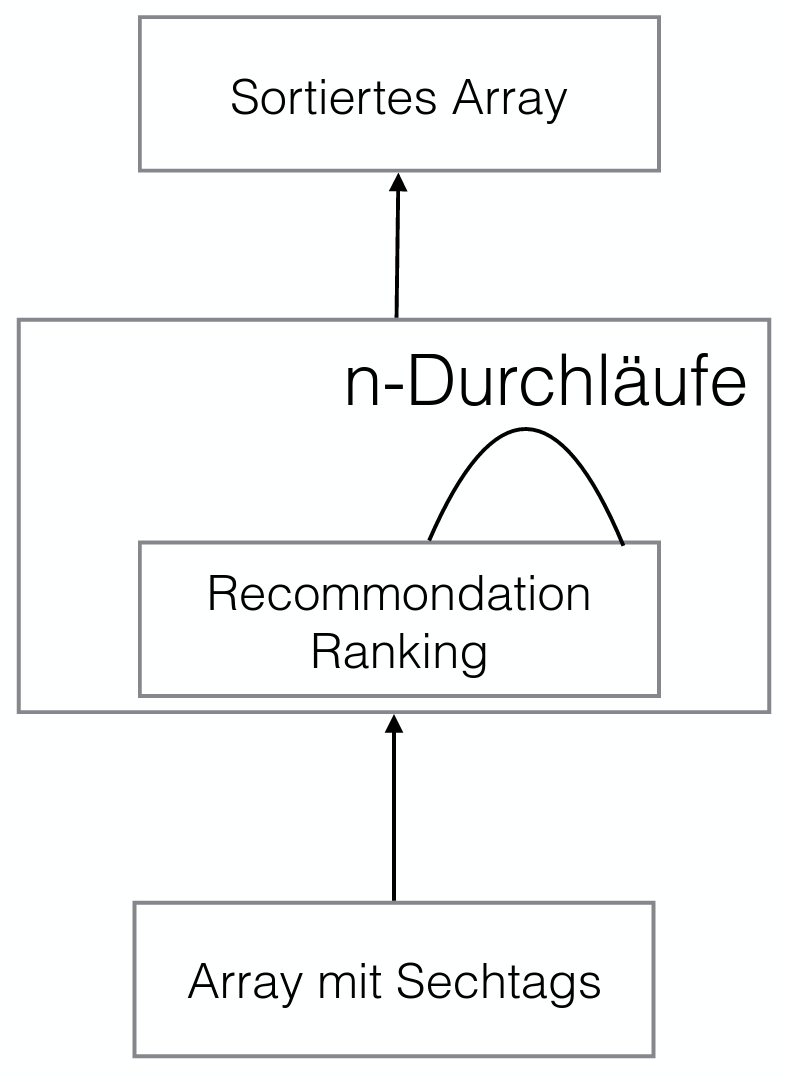
\includegraphics[width=12cm]{Pics/rankinguebersicht}

Dieses Diagramm stellt den allgemeinen Ablauf des Rankings dar. Im Folgenden wird das Recommendation Ranking im Detail erklärt. 
\newpage
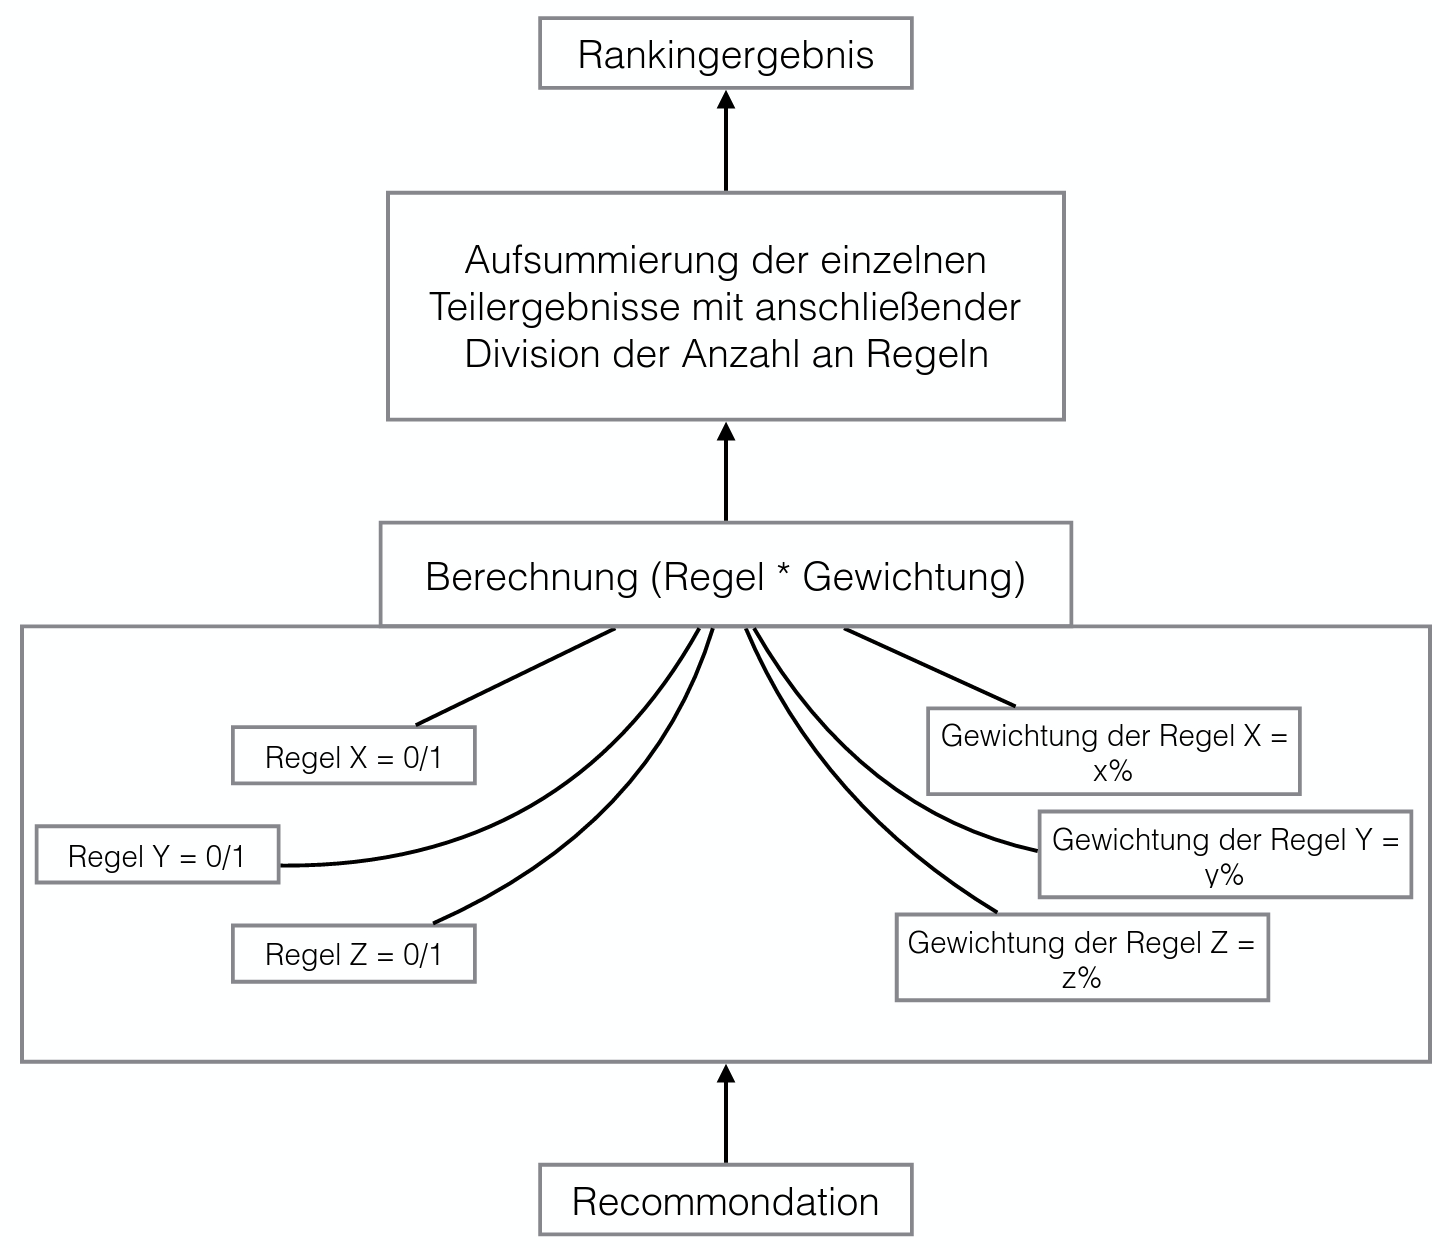
\includegraphics[width=12cm]{Pics/Ranking_Detail}

%opening
\title{Recherche der Provider und Partner}
\author{Burak Erol, Gottfried von Recum}


\chapter{Recherche der Partner und Provider}

Die Recherche zeigt auf zwei verschiedenen Excel-Dokumenten eine Liste aller Partner und Provider die für die Suchabfragen des Browsers kontaktiert werden. Es wird aufgelistet was die Webseite Inhaltlich spiegelt. Die Dokumente sollen eine Übersicht dieser Seiten für die Suchabfragen zeigen. Die Webseiten unterscheiden sich im Kontext, denn es befinden sich sowohl wissenschaftliche, technische, kulturelle als auch Personen spezifische Inhalte auf diesen verschiedenen Providern.

\begin{table}[h]
	\centering
	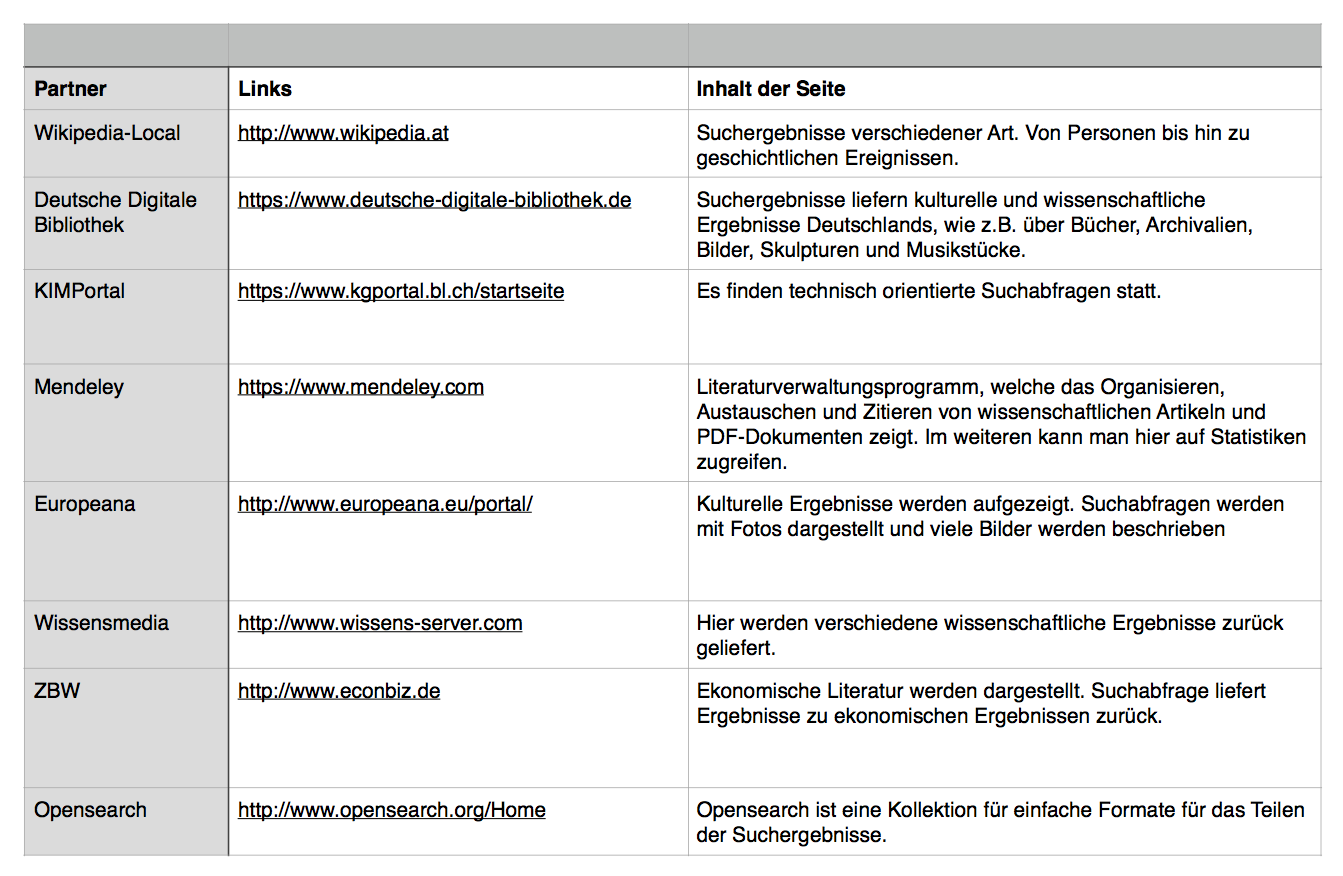
\includegraphics[width=12cm]{PartnerList}
	\caption{Liste der Partner}
	\label{fig:Partner}
\end{table}

\begin{table}[h]
	\centering
	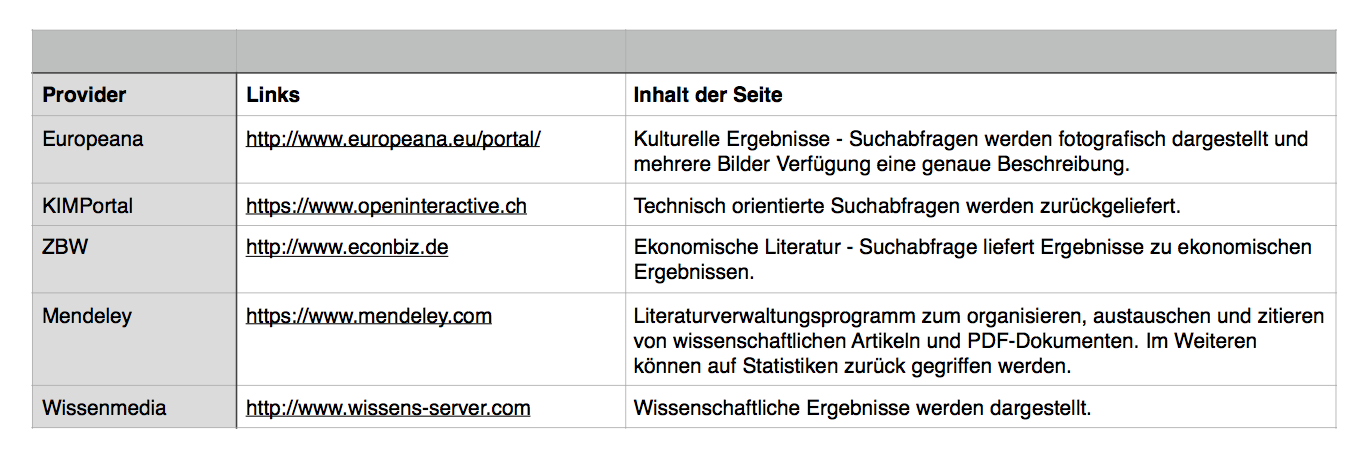
\includegraphics[width=12cm]{Pics/ProviderList}
	\caption{Liste der Provider}
	\label{fig:Provider}
\end{table}
\chapter{Testen der Applikation}

\section{Einleitung}

Zum Testen der Applikation \SECH-Browser ist es erforderlich, die in einer exemplarisch erzeugten Webseite (www.sech-browser.de/tests) eingebetteten \SEARCH-Tags zu überprüfen. Um idealerweise alle Problemfelder bzw. Fehler der App erkennen zu können, ist es erforderlich eine bestmögliche Abdeckung aller möglichen Testfälle zu gewährleisten.  

\section{Testfälle} 

Um eine bestmögliche Überprüfung der App zu erreichen, wurde eine systematische Implementierung aller denkbaren Testfälle unter \url{http://www.sech-browser.de/old-index.html} vorgenommen. Wie aus der Definition der \SEARCH-Tags ersichtlich, besteht das \SEARCH-Tag aus den drei Teilen:

\begin {itemize} 
   \item \SEARCH-Head
   \item \SEARCH-Section
   \item \SEARCH-Link
\end {itemize}

Weiterhin kann jeder Teil des \SEARCH-Tags bis zu 5 Attribute enthalten:

\begin {itemize}
   \item topic
   \item type
   \item media-type
   \item provider
   \item licence
\end {itemize}

Um alle möglichen realisierten Kombinationen der Teile der \SEARCH-Tags mit den zugehörigen Attributen aufrufen zu können, wurde eine übersichtliche Menüstruktur gewählt. Zusätzlich wurden im letzten Menüpunkt 'Fehler' noch syntaktische Fehler in den Tags eingebaut, wie Weglassen von Tag-Klammern sowie Weglassen von Anführungszeichen bei Attributen oder falsch geschriebene Attributnamen.   
Die Menü-Struktur der Testfälle ist nachfolgend dargestellt:

\pagebreak

\centering \textbf{{\large Menü -- Testfälle}}

% ----------- Hauptmenu ------------------

% ---------- keine search-tags --------------------

\flushleft \textbf{keine \SEARCH-Tags}

% ---------- search-head --------------------

\flushleft \textbf{nur \SEARCH-Head}
\begin{enumerate}
   \item mit allen Attributen
   \item mit einzelnen Attributen  
   
   \begin{enumerate}  % einzelne Attribute        
        \item nur Topic  
        \begin{itemize}
           \item mit Umlauten
           \item mit Leerzeichen
           \item mit Sonderzeichen
           \item mit Ziffern
        \end{itemize}
     
        \item nur Type
        \begin{itemize}
           \item mit Umlauten
           \item mit Leerzeichen
           \item mit Sonderzeichen
           \item mit Ziffern
        \end{itemize}
	
        \item nur mediaType
        \begin{itemize}
           \item mit Umlauten
           \item mit Leerzeichen
           \item mit Sonderzeichen
           \item mit Ziffern
        \end{itemize}
  
        \item nur Provider
        \begin{itemize}
           \item mit Umlauten
           \item mit Leerzeichen
           \item mit Sonderzeichen
           \item mit Ziffern
        \end{itemize}
  
        \item nur Licence
        \begin{itemize}
           \item mit Umlauten
           \item mit Leerzeichen
           \item mit Sonderzeichen
           \item mit Ziffern
        \end{itemize}
    \end{enumerate} % einzelne Attribute
    \item mit mehreren Attributen
    \begin{enumerate}
        \item Topic, Type
	     \item Topic, Type, mediaType
	     \item Topic, Type, mediaType, Provider
     \end{enumerate}
  \end{enumerate} % search-head



\pagebreak

% ---------- search-section --------------------

\flushleft \textbf{nur \SEARCH-Section}

\begin{enumerate}
  \item mit allen Attributen
  \item mit einzelnen Attributen

   \begin{enumerate}
    \item nur Topic  
    \begin{itemize}
    \item mit Umlauten
    \item mit Leerzeichen
    \item mit Sonderzeichen
    \item mit Ziffern
\end{itemize}
	\item nur Type
 	\begin{itemize}
    \item mit Umlauten
    \item mit Leerzeichen
    \item mit Sonderzeichen
    \item mit Ziffern
\end{itemize}
	\item nur mediaType
	\begin{itemize}
    \item mit Umlauten
    \item mit Leerzeichen
    \item mit Sonderzeichen
    \item mit Ziffern
    \end{itemize}
    \item nur Provider
	\begin{itemize}
    \item mit Umlauten
    \item mit Leerzeichen
    \item mit Sonderzeichen
    \item mit Ziffern
    \end{itemize}
    \item nur Licence
	\begin{itemize}
    \item mit Umlauten
    \item mit Leerzeichen
    \item mit Sonderzeichen
    \item mit Ziffern
    \end{itemize}
\end{enumerate}
\item mit mehereren Attributen
\begin{enumerate}
    \item Topic, Type
	\item Topic, Type, mediaType
	\item Topic, Type, mediaType, Provider
    \end{enumerate}
\end{enumerate}

\pagebreak

% ---------- search-link --------------------

\flushleft \textbf{nur \SEARCH-Link}

\begin{enumerate}
  \item mit allen Attributen
  \item mit einzelnen Attributen

   \begin{enumerate}
    \item nur Topic  
    \begin{itemize}
    \item mit Umlauten
    \item mit Leerzeichen
    \item mit Sonderzeichen
    \item mit Ziffern
\end{itemize}
	\item nur Type
 	\begin{itemize}
    \item mit Umlauten
    \item mit Leerzeichen
    \item mit Sonderzeichen
    \item mit Ziffern
\end{itemize}
	\item nur mediaType
	\begin{itemize}
    \item mit Umlauten
    \item mit Leerzeichen
    \item mit Sonderzeichen
    \item mit Ziffern
    \end{itemize}
    \item nur Provider
	\begin{itemize}
    \item mit Umlauten
    \item mit Leerzeichen
    \item mit Sonderzeichen
    \item mit Ziffern
    \end{itemize}
    \item nur Licence
	\begin{itemize}
    \item mit Umlauten
    \item mit Leerzeichen
    \item mit Sonderzeichen
    \item mit Ziffern
    \end{itemize}
\end{enumerate}
\item mit mehreren Attributen
\begin{enumerate}
    \item Topic, Type
	 \item Topic, Type, mediaType
	 \item Topic, Type, mediaType, Provider
\end{enumerate}
\end{enumerate}

\pagebreak

% ------------- search-head und search-section ----------------------

\textbf{\SEARCH-Head und \SEARCH-Section} 
\begin{enumerate}
 	\item Standard
  	\item mit Umlauten
	\item mit Leerzeichen
	\item mit Sonderzeichen
	\item mit Ziffern
\end{enumerate}

% ------------- search-head und search-link ----------------------

\textbf{\SEARCH-Head und \SEARCH-Link} 
\begin{enumerate}
   \item Standard
   \item mit Umlauten
   \item mit Leerzeichen
   \item mit Sonderzeichen
   \item mit Ziffern
\end{enumerate}

% ------------- search-section und search-link ----------------------

\textbf{\SEARCH-Section und \SEARCH-Link} 
\begin{enumerate}
   \item Standard
   \item mit Umlauten
   \item mit Leerzeichen
   \item mit Sonderzeichen
   \item mit Ziffern
\end{enumerate}


% ------------- search-head, search-section und search-link ----------------------

\textbf{\SEARCH-Head, \SEARCH-Section, \SEARCH-Link}
\begin{enumerate}
   \item Standard
   \item mit Umlauten
   \item mit Leerzeichen
   \item mit Sonderzeichen
   \item mit Ziffern
\end{enumerate}

\pagebreak

\textbf{{\large Fehler}}

\textbf{nur \SEARCH-Head}
\begin{enumerate}
\item Anführungszeichen vorne fehlt
\item Anführungszeichen hinten fehlt
\item Tag-Klammer vorne fehlt
\item Tag-Klammer hinten fehlt
\end{enumerate}

\textbf{nur \SEARCH-Section}
\begin{enumerate}
\item Anführungszeichen vorne fehlt
\item Anführungszeichen hinten fehlt
\item Beginn Tag-Klammer vorne fehlt
\item Beginn Tag-Klammer hinten fehlt
\item Ende Tag-Klammer vorne fehlt
\item Ende Tag-Klammer hinten fehlt
\end{enumerate}

\textbf{nur \SEARCH-Link}
\begin{enumerate}
\item Anführungszeichen vorne fehlt
\item Anführungszeichen hinten fehlt
\item Beginn Tag-Klammer vorne fehlt
\item Beginn Tag-Klammer hinten fehlt
\item Ende Tag-Klammer vorne fehlt
\item Ende Tag-Klammer hinten fehlt
\end{enumerate}

\textbf{\SEARCH-Head und \SEARCH-Section} 
\begin{enumerate}
\item \SEARCH-Head Topic Anführungszeichen vorne fehlt
\item \SEARCH-Section Topic Anführungszeichen hinten fehlt
\item \SEARCH-Head Tag-Klammer vorne fehlt
\item \SEARCH-Section Beginn Tag-Klammer hinten fehlt
\item \SEARCH-Section Ende Tag-Klammer hinten fehlt
\item \SEARCH-Section nicht geschlossen
\end{enumerate}

\pagebreak
\textbf{\SEARCH-Head und \SEARCH-Link} 
\begin{enumerate}
\item \SEARCH-Head Topic Anführungszeichen vorne fehlt
\item \SEARCH-Link Topic Anführungszeichen hinten fehlt
\item \SEARCH-Head Tag-Klammer vorne fehlt
\item \SEARCH-Link Beginn Tag-Klammer hinten fehlt
\item \SEARCH-Link Ende Tag-Klammer hinten fehlt
\item \SEARCH-Link nicht geschlossen
\end{enumerate}

\textbf{\SEARCH-Section und \SEARCH-Link} 
\begin{enumerate}
\item \SEARCH-Section Topic Anführungszeichen vorne fehlt
\item \SEARCH-Link Topic Anführungszeichen hinten fehlt
\item \SEARCH-Section Tag-Klammer vorne fehlt
\item \SEARCH-Section Ende  Tag-Klammer hinten fehlt
\item \SEARCH-Section nicht geschlossen
\item \SEARCH-Link Beginn Tag-Klammer hinten fehlt
\item \SEARCH-Link Ende  Tag-Klammer hinten fehlt
\item \SEARCH-Link nicht geschlossen
\end{enumerate}

\textbf{\SEARCH-Head, \SEARCH-Section, \SEARCH-Link}

\begin{enumerate}
\item \SEARCH-Head falscher Attributname (topics statt topic)
\item \SEARCH-Section falscher Attributname (provide statt provider)
\item \SEARCH-Link falscher Attributname (license statt licence)
\item \SEARCH-Head Tag-Klammer vorne fehlt
\item \SEARCH-Section Tag-Klammer vorne fehlt
\item \SEARCH-Section Ende  Tag-Klammer hinten fehlt
\item \SEARCH-Section nicht geschlossen
\item \SEARCH-Link Beginn Tag-Klammer vorne fehlt
\item \SEARCH-Link Ende  Tag-Klammer hinten fehlt
\item \SEARCH-Link nicht geschlossen
\end{enumerate}

\section{Auswertung der Testfälle}

Sobald nur ein \SEARCH-Head vorhanden ist, wird dieser nicht ausgewertet und es werden keine \SEARCH-Links angezeigt.

Sobald nur eine oder mehrere \SEARCH-Sections vorhanden sind, werden diese nicht ausgewertet und es werden keine \SEARCH-Links angezeigt.

Sobald \SEARCH-Links vorhanden sind, werden diese entsprechend ausgewertet und sie werden korrekt in der TableView der \SEARCH-Tags angezeigt.

Es treten Fehler auf, sobald im \SEARCH-Link die Anführungszeichen fehlen, denn es werden trotzdem entsprechende \SEARCH-Links gefunden und fehlerhaft angezeigt.

Sobald \SEARCH-Tag-Klammern fehlen, können diese nicht ausgewertet werden und werden nicht angezeigt.

%opening
\title{WkWebView JavaScript}
\author{Andreas Netsch}



\section{ WkWebKit JavaScript}

WkWebKit ersetzt den ursprünglichen UIWebView und wurde in unserer App nachträglich hinzugefügt, da war anfangs einen UIWebView verwendet haben. Dieser bietet aber weniger funktionen und wird somit von Apple nicht mehr empfohlen. Die Einbindung des WkWebView ist zum derzeitigen Stand jedoch noch nicht über den Interface Builder möglich und muss somit programatisch erstellt werden.
Erzeugen der verwendeten Variable myWebView als WKWebView:
\begin{verbatim}
var myWebView: WKWebView?
\end{verbatim}
Zuweisung des WebViewDelegates ind er Funktion viewDidLoad():
\begin{verbatim}
myWebViewDelegate = WebViewDelegate()
myWebViewDelegate.viewCtrl = self
\end{verbatim}
Um JavaScript in die WkWebView einzubinden muss eine WkWebViewConfiguration erstellt werden:
\begin{verbatim}
let config = WKWebViewConfiguration()
\end{verbatim}
Als nächstes muss der Pfad der JavaScript Datei angegeben werden mit dieser wird der ScriptContent extrahiert. Des weiteren muss der Zeitpunkt des Einfügens in das Dokument angegeben werden. Dies wird der WkWebViewConfiguration hinzugefügt genauso wie ein ScriptMessageHandler der auf klick Ereignisse reagiert:
\begin{verbatim}
let scriptURL = NSBundle.mainBundle().pathForResource("main", ofType:
 "js")
 
let scriptContent = try! String( contentsOfFile: scriptURL!, encoding:
NSUTF8StringEncoding)

let script = WKUserScript(source: scriptContent, injectionTime: 
.AtDocumentStart, forMainFrameOnly: true)

config.userContentController.addUserScript(script)
        
config.userContentController.addScriptMessageHandler(self, name:
 "onclick")
\end{verbatim}
Die WkWebViewConfiguration hat nun alle erforderlichen Komponenten und kann zusammen mit der Angabe des Frames welcher hier die Grenzen des ContinerViews sind als SubView des ContainerViews gesetzt werden:
\begin{verbatim}

self.myWebView = WKWebView(frame: containerView.bounds,
configuration: config)
self.containerView.addSubview(myWebView!)
\end{verbatim}


\pagebreak


\end{document}
